  \documentclass[12pt,oneside]{article}

%%%%%%%%%%%%%%%%%%%%%%%%%%%%
%%   Zusaetzliche Pakete  %%
%%%%%%%%%%%%%%%%%%%%%%%%%%%%
\usepackage{acronym}
\usepackage{enumerate}
\usepackage{a4wide}
\usepackage{fancyhdr}
\usepackage{graphicx}
\usepackage{palatino}
\usepackage{blindtext}
\usepackage{multirow}
\usepackage[ruled,longend]{algorithm2e}
\usepackage{float}
\usepackage{amsmath}
\usepackage{amssymb}
\usepackage{listings}
\usepackage{tocbibind}
\usepackage{dirtytalk}
%folgende Zeile auskommentieren für englische Arbeiten
\usepackage[ngerman]{babel}
 \usepackage[utf8]{inputenc}
\usepackage{enumitem}
\usepackage[bookmarks]{hyperref}
\usepackage[T1]{fontenc}
\usepackage[utf8]{inputenc}
\usepackage[a-1b]{pdfx}
\usepackage[justification=centering]{caption}
%\usepackage[style=unsrt,natbib=true,backend=biber]{biblatex}
\usepackage{csquotes}
\usepackage{url}
%\usepackage{subfigure}
\usepackage[utf8]{inputenc}
\usepackage[T1]{fontenc}
\usepackage{listings}
\usepackage{xcolor}
% Layout corrections (Schusterjungen)
\clubpenalty = 10000 
% Layout corrections (Hurenkinder) 
\widowpenalty = 10000 
\displaywidowpenalty = 10000

% Figures
\usepackage{caption}
\usepackage[hypcap=true,labelformat=simple]{subcaption}
\renewcommand{\thesubfigure}{(\alph{subfigure})}
\usepackage{wrapfig}
% Tables
\usepackage{booktabs} 
 
\usepackage[backend=biber,style=numeric]{biblatex}
\addbibresource{literatur.bib}


% Newcommand TODO (red in text)
\newcommand{\todo}[1]{\textcolor{red}{TODO: #1}}

% Newcommand TODOM (red at border)
\newcommand{\todom}[1]{\marginpar{\parbox{1.5cm}{\textcolor{red}{TODO:\\ #1}}}}
\lstset{
  literate=%
    {ö}{{\"o}}1
    {ü}{{\"u}}1
    {ä}{{\"a}}1
    {Ö}{{\"O}}1
    {Ü}{{\"U}}1
    {Ä}{{\"A}}1
}

\lstdefinestyle{java}{
    language=Java,
    basicstyle=\ttfamily\small,
    keywordstyle=\color{blue},
    stringstyle=\color{red},
    commentstyle=\color{green},
    numbers=left,
    numberstyle=\tiny,
    stepnumber=1,
    breaklines=true,
    frame=single,
    tabsize=4
}

\lstdefinestyle{sql}{
    language=SQL,
    basicstyle=\ttfamily\small,
    keywordstyle=\color{purple},
    stringstyle=\color{orange},
    commentstyle=\color{green},
    numbers=left,
    numberstyle=\tiny,
    stepnumber=1,
    breaklines=true,
    frame=single,
    tabsize=4
}
\lstdefinestyle{typescript}{
    language=TypeScript,
    basicstyle=\ttfamily\small,
    keywordstyle=\color{blue},
    stringstyle=\color{orange},
    commentstyle=\color{green},
    numbers=left,
    numberstyle=\tiny,
    stepnumber=1,
    breaklines=true,
    frame=single,
    tabsize=4,
    morekeywords={let, const, async, await, interface, type, readonly, enum, export, extends, implements, private, public, protected, static, declare, namespace},
}
\lstdefinelanguage{HTML}{
    language=HTML,
    sensitive=true,
    alsoletter={<>=-},
    morecomment=[s]{<!--}{-->},
    morestring=[b]",
    morestring=[s]{'}{'},
    tagstyle=\color{blue},
    stringstyle=\color{red},
    commentstyle=\color{gray},
}

\lstdefinelanguage{TypeScript}{
    language=JavaScript,
    morekeywords={type,interface,implements,public,private},
    keywordstyle=\color{blue},
    stringstyle=\color{red},
    commentstyle=\color{green},
    numbers=left,
    numberstyle=\tiny,
    stepnumber=1,
    breaklines=true,
    frame=single,
    tabsize=4
}

 

%%%%%%%%%%%%%%%%%%%%%%%%%%%%%%
%% Definition der Kopfzeile %%
%%%%%%%%%%%%%%%%%%%%%%%%%%%%%%

\pagestyle{fancy}
\fancyhf{}
\cfoot{\thepage}
\setlength{\headheight}{16pt}

%%%%%%%%%%%%%%%%%%%%%%%%%%%%%%%%%%%%%%%%%%%%%%%%%%%%%
%%  Definition des Deckblattes und der Titelseite  %%
%%%%%%%%%%%%%%%%%%%%%%%%%%%%%%%%%%%%%%%%%%%%%%%%%%%%%

\newcommand{\HSFTitle}[8]{

  \thispagestyle{empty}
\begin{center}
    
\includegraphics[width=0.8\textwidth]{logo.eps} \\
    \vspace*{\stretch{1}}
\end{center}

  %\vspace*{\stretch{1}}
  {\parindent0cm
  \rule{\linewidth}{.7ex}}
  \begin{center}
    \vspace*{\stretch{1}}
    \sffamily\bfseries\Huge
    #1\\
    \vspace*{\stretch{1}}
    \sffamily\bfseries\large
    #3
    \vspace*{\stretch{1}}
  \end{center}
  \rule{\linewidth}{.7ex}

  \vspace*{\stretch{2}}
  \begin{center}
    \Large #2 am #5 der HAW Fulda \\
    \vspace*{\stretch{1}} 
    \large Matrikelnummer:  #4 \\[1mm]
    \large Erstbegutachtung:  #7 \\[1mm]
    \large Zweitbegutachtung:  #8 \\[1mm]
    \vspace*{\stretch{1}}
    \large Eingereicht am #6
  \end{center}
}


%%%%%%%%%%%%%%%%%%%%%%%%%%%%
%%  Beginn des Dokuments  %%
%%%%%%%%%%%%%%%%%%%%%%%%%%%%


\begin{document}
 
 

 \HSFTitle
      {Entwicklung und Implementierung eines Modells zur Erfassung und Bewertung der User Experience am Beispiel der Anwendung eDok des LWV Hessen }        % Titel der Arbeit
      {Bachelorarbeit} % Typ der Arbeit
      {Ali Alkhiami}          % Vor- und Nachname des Autors
      {844620}
      {Fachbereich AI}  % Name des FBs
      {05.mm.yyyy}        % Tag der Abgabe
      {Prof. Dr. Alexander Gepperth}     % Name des Erstgutachters
      {Prof. Dr. Dr. YYY}    % Name des Zweitgutachters

  \clearpage

\lhead{}
    \setcounter{page}{1}
%--------------------------------------------------------------------------------------------------------------------------------------------------------------------------------------%
 

\subsection{Abstract}

Diese Arbeit befasst sich mit der Entwicklung und Implementierung eines Modells zur umfassenden Erfassung und Bewertung der User Experience (UX), exemplarisch angewendet auf die Anwendung eDok des Landeswohlfahrtsverbands Hessen (LWV Hessen). Ziel des Modells ist es, einen detaillierten Überblick über die UX innerhalb der Anwendung zu schaffen, indem während der produktiven Nutzung anonymisierte Daten gesammelt werden.

Die gesammelten Daten sind bewusst nicht benutzerorientiert, um Datenschutzrichtlinien einzuhalten und die Privatsphäre der Nutzer zu schützen. Das Modell präsentiert diese aggregierten Daten in einem Dashboard, das ausschließlich für Nutzer mit Administratorrechten zugänglich ist. Dieses Dashboard bietet anpassbare Grafiken und Visualisierungen, die durch Filter und weitere Kriterien modifiziert werden können. Dadurch erhalten Administratoren nicht nur Einblicke in die aktuelle UX, sondern können auch Trends und Entwicklungen über einen bestimmten Zeitraum analysieren.

Ein wesentlicher Aspekt des Modells ist die Möglichkeit für Projektverantwortliche, die Datenerfassung auf bestimmten Seiten der Anwendung gezielt an- oder auszuschalten. Dies stellt sicher, dass nur relevante Bereiche beobachtet werden, ohne die Performance auf anderen Seiten zu beeinträchtigen. Das Modell ermöglicht es, die Verweildauer der Nutzer auf spezifischen Seiten zu überwachen, häufig durchlaufene Navigationsmuster zu identifizieren und die Häufigkeit bestimmter Fehler zu erfassen, die von den Nutzern gemacht werden.

Die gewonnenen Erkenntnisse unterstützen die Projektverantwortlichen dabei, problematische Stellen innerhalb der Anwendung zu identifizieren und gezielte Maßnahmen zur Verbesserung der Usability zu ergreifen. Darüber hinaus ermöglicht das Modell eine nachträgliche Überprüfung der implementierten Änderungen, um deren Effektivität zu bewerten und weitere Optimierungen vorzunehmen. Durch diesen iterativen Prozess trägt das Modell wesentlich zur Steigerung der Benutzerzufriedenheit und Effizienz der Anwendung bei.

%--------------------------------------------------------------------------------------------------------------------------------------------------------------------------------------%
\tableofcontents
%--------------------------------------------------------------------------------------------------------------------------------------------------------------------------------------%
 
 
\addcontentsline{toc}{subsection}{Abkürzungsverzeichnis} % Fügt das Abkürzungsverzeichnis zum Inhaltsverzeichnis hinzu
\begin{acronym}[hyperlinks]
\acro{UX}{User Experience}
\acro{LWV}{Landeswohlfahrtsverband}
\acro{SUS}{System Usability Scale}
\acro{UEQ}{User Experience Questionnaire}
\acro{UI}{User Interface}
\acro{eDok}{elektronische Dokumentenerstellung}
\acro{HCI}{Humin Computer Interaction}
\end{acronym}

\section{Einleitung}

Die \textbf{Mensch-Computer-Interaktion} (Human-Computer Interaction, HCI) ist ein interdisziplinäres Forschungsfeld, das sich mit der Gestaltung, Evaluation und Implementierung interaktiver Computersysteme für die menschliche Nutzung sowie mit der Untersuchung der damit verbundenen Phänomene beschäftigt. Innerhalb dieses Feldes haben sich zwei zentrale Ansätze zur \textbf{User Experience} (UX) herausgebildet: das \textbf{UX-Design} und das \textbf{nutzerzentrierte Design} (User-Centered Design) \cite{glanznig}.

Das \textbf{UX-Design} strebt danach, ein ganzheitliches Nutzererlebnis zu schaffen, das über die reine Funktionalität eines Produkts hinausgeht. Es berücksichtigt emotionale, psychologische und ästhetische Aspekte, um Produkte zu entwickeln, die nicht nur effizient, sondern auch angenehm und zufriedenstellend in der Nutzung sind. Ziel ist es, ein positives Gesamterlebnis zu gestalten, das die Bedürfnisse und Erwartungen der Nutzer übertrifft.

Im Gegensatz dazu fokussiert das \textbf{nutzerzentrierte Design} auf die Einbindung der Endnutzer während des gesamten Entwicklungsprozesses. Durch aktive Einbindung von Nutzerfeedback wird sichergestellt, dass das Endprodukt intuitiv bedienbar ist und den Anforderungen der Zielgruppe entspricht. Dieser Ansatz betont die Bedeutung, die tatsächlichen Bedürfnisse, Ziele und Fähigkeiten der Nutzer zu verstehen und in die Gestaltung einzubeziehen.

Obwohl beide Ansätze entscheidend für die Entwicklung qualitativ hochwertiger Produkte sind, liegt der Schwerpunkt dieser Arbeit nicht auf der Gestaltung selbst, sondern darauf, \textbf{wie UX erfasst und gemessen werden kann}. In einer zunehmend digitalisierten Welt, in der Anwendungen immer komplexer werden und die Erwartungen der Nutzer stetig steigen, ist die systematische Messung der UX von entscheidender Bedeutung. Nur durch ein tiefgehendes Verständnis des Nutzerverhaltens und der Nutzerzufriedenheit können Produkte entwickelt werden, die den hohen Ansprüchen gerecht werden.
\subsection{Kontext}
\begin{wrapfigure}{r}{0.4\textwidth} % 'r' for right, width of the figure
    
\includegraphics[width=0.3\textwidth]{lwv.png} % Adjust the width as needed
\end{wrapfigure}
Der \textbf{Landeswohlfahrtsverband Hessen} (LWV Hessen) ist eine zentrale Organisation, die als überörtlicher Träger der Eingliederungshilfe tätig ist. Er fördert die soziale Integration und Unterstützung von Menschen mit Behinderungen in Bereichen wie Wohnen, Bildung, Mobilität und Arbeit. Mit der Umsetzung des Bundesteilhabegesetzes sowie Programmen wie dem \textit{Persönlichen Budget} und dem \textit{Budget für Arbeit} ermöglicht der Verband eine selbstbestimmte Lebensführung und gesellschaftliche Teilhabe. Zusätzlich bietet der LWV Hessen spezifische Förderangebote für Kinder und Jugendliche mit geistigen, emotionalen oder körperlichen Einschränkungen, darunter Frühberatungsstellen und Förderschulen. Auch Menschen, die Leistungen des Sozialen Entschädigungsrechts benötigen, finden beim LWV Hessen Unterstützung.
\begin{wrapfigure}{r}{0.3\textwidth} % 'r' for right, width of the figure
    
\includegraphics[width=0.3\textwidth]{anlei.png} % Adjust the width as needed
\end{wrapfigure}
Die \textbf{ANLEI-Service GmbH}, eine Tochtergesellschaft des LWV Hessen, ergänzt dessen Tätigkeiten durch IT-Dienstleistungen für die Sozialverwaltung. Sie entwickelt Systeme zur Unterstützung von Antragsbearbeitung, Leistungsgewährung und Abrechnung von Sozialleistungen, insbesondere in den Bereichen Eingliederungshilfe, Sozialhilfe und Kriegsopferfürsorge. Zu den zentralen Anwendungen gehören das \textit{Integrierte Berichtssystem} (IBS) für betriebswirtschaftliche Analysen und \textit{MASS}, das die maschinelle Abrechnung mit Einrichtungen und Trägern erleichtert.

Ein weiterer wichtiger Bestandteil ist \textit{eDok}, ein moderner Service für die Erstellung barrierefreier Dokumente, der das bisherige \textit{Schriftstück-Erstellungssystem} (SE) ablöst, das auf Microsoft Word und Makros basierte. \textit{eDok} integriert \textit{Doxee/Infinica} als Subsystem für die Dokumentbearbeitung und Output-Generierung, was sowohl eine interaktive Bearbeitung der Dokumente als auch eine automatisierte Verarbeitung im Hintergrund ermöglicht. Ziel ist es, eine universelle und generische Schnittstelle für die Anwendungen des LWV Hessen bereitzustellen, die eine einfache, effiziente und performante Erstellung barrierefreier Dokumente sicherstellt und die Daten aus den Fachverfahren nahtlos einbezieht.

Diese Bachelorarbeit wird im Rahmen einer praktischen Zusammenarbeit mit dem \textbf{LWV Hessen} erstellt. Ziel ist es, ein innovatives System zu entwickeln, das Nutzungsdaten anonymisiert erfasst.
Diese Arbeit verbindet praxisorientierte Softwareentwicklung mit wissenschaftlicher Forschung und trägt dazu bei, die Usability und Effizienz der Anwendung \textit{eDok} zu optimieren.

Durch die direkte Einbindung in die Arbeitsprozesse des LWV Hessen wird nicht nur die Relevanz des Themas unterstrichen, sondern es entsteht auch eine wertvolle Gelegenheit, die entwickelten Konzepte und Technologien in einer realen Umgebung zu testen und anzuwenden. Somit leistet diese Arbeit einen Beitrag zur Verbesserung der digitalen Arbeitsabläufe des LWV Hessen und zur praxisnahen Weiterentwicklung moderner UX-Methoden.
\subsection{Relevanz der Arbeit}

Angesichts der wachsenden Bedeutung von UX in der Softwareentwicklung leistet diese Arbeit einen wichtigen Beitrag zur Praxis und Forschung. Das vorgestellte Modell ermöglicht es, UX-Daten in Echtzeit und unter realen Nutzungsbedingungen zu erfassen, ohne die Nutzererfahrung zu beeinträchtigen. Dies ist besonders relevant für Organisationen, die ihre Anwendungen kontinuierlich verbessern möchten, um den steigenden Erwartungen der Nutzer gerecht zu werden.

Durch die Anwendung auf die \textit{eDok}-Anwendung des LWV Hessen wird demonstriert, wie das Modell in einer realen Umgebung implementiert werden kann. Die gewonnenen Erkenntnisse können als Grundlage für weitere Anwendungen dienen und dazu beitragen, die UX-Forschung in der Praxis voranzutreiben.
\subsection{Motivation}

Die rasante technologische Entwicklung und die immer stärkere Integration des Internets in den Alltag haben die Art und Weise, wie Menschen mit digitalen Systemen interagieren, grundlegend verändert. Laut der ARD/ZDF-Onlinestudie \cite{ard} nutzen mittlerweile rund 90 Prozent der deutschsprachigen Bevölkerung ab 14 Jahren regelmäßig das Internet, wobei insbesondere die mediale Internetnutzung in den letzten Jahren signifikant zugenommen hat. Diese Entwicklung stellt neue Anforderungen an die Gestaltung von Nutzererlebnissen und unterstreicht die Bedeutung einer herausragenden UX.

In diesem Kontext wird es immer wichtiger, digitale Inhalte und Dienste so zu gestalten, dass sie den sich wandelnden Ansprüchen der Nutzer gerecht werden. Anwendungen müssen nicht nur funktional sein, sondern auch intuitiv bedienbar und ästhetisch ansprechend gestaltet sein, um im Wettbewerb bestehen zu können. Dies gilt insbesondere für komplexe Webanwendungen wie \textit{eDok}, die von Institutionen wie dem LWV Hessen genutzt werden.

Eine besondere Herausforderung besteht darin, innerhalb solcher Anwendungen Bereiche zu identifizieren, die ein verbessertes Design oder zusätzliche Informationen erfordern. Nutzer können unsicher sein, wie sie ihre Ziele innerhalb der Anwendung erreichen können, oder sich von der Informationsmenge überfordert fühlen. Hier setzt das entwickelte Modell an, das die UX automatisiert erfasst und eine fundierte Analyse ermöglicht. So können gezielt Schlüsselaspekte identifiziert werden, die optimiert werden sollten, um die Nutzerzufriedenheit zu steigern.

Zudem führen die regelmäßige Einführung neuer Funktionen und Veränderungen in der Benutzeroberfläche zu einer dynamischen Komplexitätsentwicklung in verschiedenen Bereichen der Anwendung. Ein Überblick über die Entwicklung der UX im Laufe der Zeit ermöglicht eine proaktive Anpassung und Optimierung, sodass die Anwendung trotz zunehmender Komplexität benutzerfreundlich bleibt.

Die wissenschaftliche Forschung betont die Wichtigkeit von Methoden zur UX-Messung und -Bewertung, um sicherzustellen, dass die Produktentwicklung in die richtige Richtung geht \cite{Virpi}. Die Fähigkeit, UX quantitativ und qualitativ zu erfassen, bietet Unternehmen und Entwicklern einen unschätzbaren Vorteil. Durch das Verständnis des Nutzerverhaltens und der Nutzerzufriedenheit können gezielte Verbesserungen vorgenommen werden, die nicht nur die Effizienz steigern, sondern auch die Bindung der Nutzer an das Produkt fördern.

\subsection{Ziel der Arbeit}

Das Hauptziel dieser Arbeit ist die Entwicklung und Implementierung eines Modells, das eine umfassende Erfassung und Bewertung der UX ermöglicht. Dieses Modell soll spezifische, anonymisierte Daten sammeln, um die UX präzise und systematisch zu erfassen. Durch die Analyse dieser Daten über Zeiträume hinweg sollen dynamische Veränderungen erkannt und gezielte Optimierungsmöglichkeiten der Anwendung erschlossen werden.

Exemplarisch wird dieses Modell auf die Anwendung \textit{eDok} des LWV Hessen angewendet. Dabei soll ein System geschaffen werden, das während der produktiven Nutzung Daten sammelt, ohne die Privatsphäre der Nutzer zu beeinträchtigen. Diese Daten werden in einem Dashboard visualisiert, das ausschließlich für Administratoren zugänglich ist, um fundierte Entscheidungen zur Optimierung der Anwendung treffen zu können.

Ein weiterer Aspekt ist die Möglichkeit für Entwickler und Produktverantwortliche, die Datenerfassung auf spezifische Seiten der Anwendung zu beschränken oder zu erweitern. Dadurch kann sichergestellt werden, dass nur relevante Bereiche beobachtet werden, ohne die Performance auf anderen Seiten zu beeinträchtigen. Zudem ermöglicht das Modell, die Effektivität von Anpassungen zu überprüfen, indem Veränderungen im Nutzerverhalten nach Implementierung von Updates sichtbar gemacht werden.

\subsection{Fragestellung}

Welche spezifischen, anonymisierten Daten sind erforderlich, um ein Modell zu entwickeln und zu implementieren, das die User Experience präzise und systematisch erfasst, dynamische Veränderungen über Zeiträume hinweg analysiert, Verantwortliche bei fundierten Entscheidungen zur Optimierung der Anwendung unterstützt und dabei auftretende Herausforderungen bewältigt?
\subsection{Eigenleistung}
Im Rahmen der vorliegenden Arbeit wurde auf keinerlei nicht-öffentliche Vorarbeiten zurückgegriffen. Sämtliche entwickelte Softwarekomponenten (Angular-Frontend, Java-Spring-Backend sowie die SQL-Datenbankstrukturen) wurden von mir selbst erstellt oder basieren ausschließlich auf frei verfügbaren bzw. quelloffenen Bibliotheken, die unter entsprechend erlaubten Lizenzen stehen ( Angular CLI, Spring Boot, SQLite).

\section{Grundlagen und Methodik}
In diesem Kapitel werden die methodischen und technischen Grundlagen vorgestellt, welche die Basis für die spätere Umsetzung im Rahmen dieser Arbeit bilden. Dabei wird auf bereits existierende Konzepte und Bibliotheken verwiesen, die im Projekt verwendet wurden. Zudem wird erläutert, wie die Datenbankstruktur und die zugrunde liegende Architektur gewählt wurden, um die Zielsetzungen der Arbeit (Erfassung, Analyse und Visualisierung von Nutzerinteraktionen) zu erfüllen. Auf detaillierte Implementierungsschritte wird hier verzichtet; diese finden sich in den folgenden Kapiteln und im Anhang.

\subsection{Architektur und Softwarekomponenten}

Die gewählte Systemarchitektur besteht aus einem Angular-Frontend und einem Spring-Boot-Backend, das auf einer relationalen Datenbank (z.\,B. SQLite) aufsetzt:

\begin{itemize}
    \item \textbf{Frontend (Angular)}
    \begin{itemize}
        \item Zuständig für die Erfassung der Nutzerinteraktionen (z.\,B. Klicks, Fehlermeldungen) und die Darstellung der Ergebnisse im Admin-Dashboard.
        \item Setzt u.\,a. auf asynchrone Service-Aufrufe und reaktive Konzepte (RxJS), um Daten in Echtzeit oder in festgelegten Intervallen zu erfassen und an das Backend zu schicken.
    \end{itemize}
    \item \textbf{Backend (Spring Boot)}
    \begin{itemize}
        \item Stellt REST-Schnittstellen zur Verfügung, die vom Frontend konsumiert werden.
        \item Übernimmt die Geschäftslogik, indem es eingehende Events (Klicks, Fehlermeldungen usw.) verarbeitet, validiert und in der Datenbank persistiert.
        \item Aggregiert die Daten (z.\,B. zur Erstellung von Heatmaps oder zur Analyse von Navigationspfaden) und sendet die Ergebnisse zurück ans Frontend.
    \end{itemize}
    \item \textbf{Datenhaltung (relationales Modell)}
    \begin{itemize}
        \item Datenbanktabellen, in denen Sitzungen (Sessions), Klick-Events, Fehler-Events und Netzwerkabfragen erfasst werden.
        \item Trennung zwischen dynamischen Nutzungsdaten (z.\,B. Klickereignissen) und statischen Entitäten (z.\,B. Komponenten-Beschreibungen), um eine klare Struktur und Erweiterbarkeit zu gewährleisten.
    \end{itemize}
\end{itemize}

Diese Aufteilung ermöglicht eine lose Kopplung zwischen Frontend und Backend sowie eine modulare Erweiterbarkeit der Datenerfassung und Analyse.

\subsection{Datenbankmodell}

Zur Speicherung und Auswertung der erhobenen Interaktionsdaten kommt ein relationales Datenmodell zum Einsatz. Wesentliche Entitäten sind:

\begin{itemize}
    \item \textbf{Usability Session}: Repräsentiert eine anonyme Sitzung und verknüpft diese mit einer konkreten Komponente (z.\,B. einem Modul der Anwendung). Enthält Start- und Endzeit sowie ein Session-Token als eindeutigen Bezeichner.
    \item \textbf{Click Event}: Zeichnet jede Klick-Interaktion innerhalb einer Session auf. Wichtige Felder sind das angeklickte UI-Element (\texttt{element\_id}), eine Sequenznummer zur Rekonstruktion der Klickfolge und ein Zeitstempel.
    \item \textbf{Error Event}: Erfasst Fehler, die während einer Session auftreten (z.\,B. Ausnahmen im Frontend oder gemeldete Fehler über ein Formular). Ermöglicht die Kategorisierung und Zählung von Fehlern, um Problembereiche zu identifizieren.
    \item \textbf{Network Request}: Speichert Informationen zu einzelnen Netzwerkaufrufen wie Startzeit, Endzeit, HTTP-Methode und ggf. Antwortstatus. Wichtig zur Performance-Analyse und zum Auffinden von Engpässen.
    \item \textbf{Component}: Enthält Metadaten zu einer (Sub-)Anwendung bzw. UI-Komponente, sodass Sitzungen und Events eindeutig zugeordnet werden können.
\end{itemize}

Dieses Datenmodell ermöglicht eine gezielte Analyse von Nutzerwegen, Klickhäufigkeiten, Fehlerursachen und Performance-Daten, ohne dabei personenbezogene Daten zu erheben. Durch die Entkopplung zwischen „Sitzungen“ und konkreten Nutzern wird die Privatsphäre gewahrt.

\subsection{Methodisches Vorgehen bei der Datenerfassung}

\begin{itemize}
    \item \textbf{Event Listener im Frontend}: In Angular-Komponenten werden Klick- und Fehlerevents über globale oder lokale Listener abgefangen. Die Daten (Element-ID, Zeitstempel, Session-Token usw.) werden minimal verarbeitet (z.\,B. Ergänzung eines Sequenzzählers) und anschließend an das Backend gesendet.
    \item \textbf{Persistierung und Anreicherung im Backend}: Das Spring-Boot-Backend nimmt die Daten entgegen, validiert sie und legt sie in den entsprechenden Tabellen ab (siehe Abschnitt \ref{sec:datenbankmodell}). Zudem können Zeitinformationen (z.\,B. \texttt{time\_since\_previous}) ergänzt oder bestehende Sessions automatisch geschlossen werden, wenn eine Inaktivität vorliegt.
    \item \textbf{Auswertung}: Um Heatmap-Daten, häufigste Pfade oder Fehlerstatistiken zu erzeugen, werden Aggregationsfunktionen und gruppierte Abfragen verwendet. Die Ergebnisse werden entweder direkt an das Frontend geliefert (z.\,B. für Live-Analysen) oder in periodischen Abständen abgerufen, um Berichte oder Dashboards zu aktualisieren.
    \item \textbf{Datenschutz}: Nur technische und kontextbezogene Daten werden gespeichert (z.\,B. Session-Token statt Nutzer-ID). Keine Speicherung von Klartext-Personendaten. Konzeption und Implementierung sind darauf ausgelegt, geltende Datenschutzvorgaben einzuhalten.
\end{itemize}

\subsection{SQL-Datenbankmodell}
\begin{figure}[htb]
  \centering
  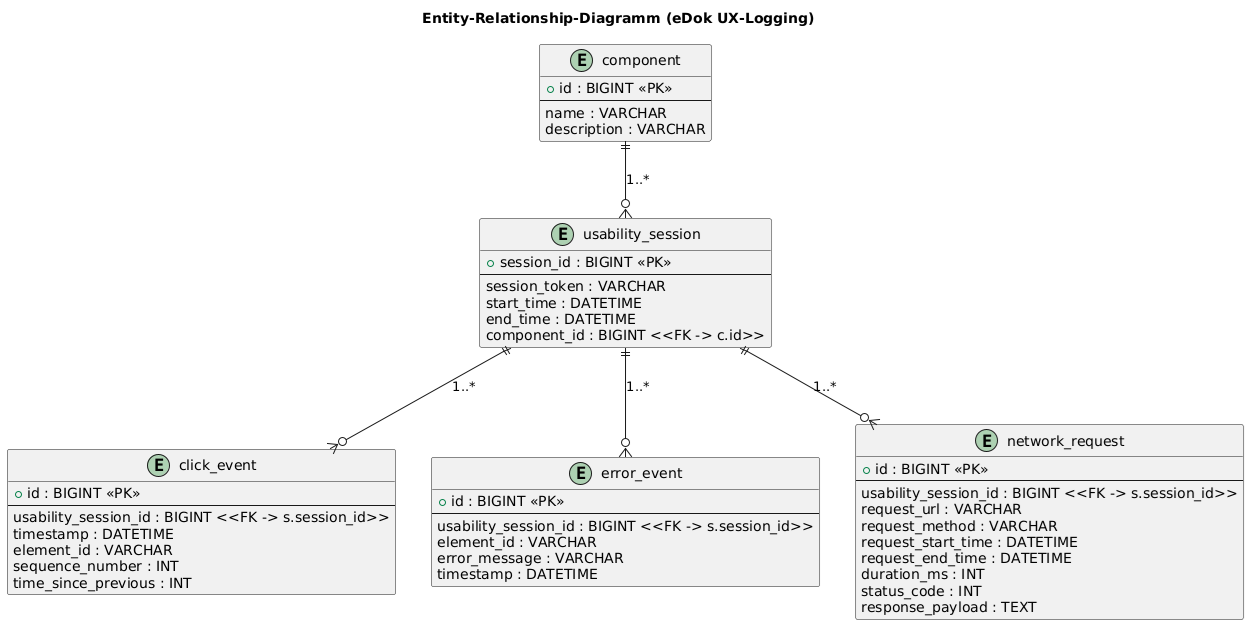
\includegraphics[width=0.85\textwidth]{erd-logging.png}
  \caption{Datenbankmodell für das eDok UX-Logging}
  \label{fig:erd-logging}
\end{figure}

\lstset{style=sql}
\begin{lstlisting}
CREATE TABLE click_event (
    id                   BIGINT NOT NULL PRIMARY KEY,
    element_id           VARCHAR(255),
    sequence_number      INTEGER NOT NULL,
    time_since_previous  INTEGER,
    timestamp            TIMESTAMP,
    usability_session_id BIGINT NOT NULL
);

CREATE TABLE component (
    id          BIGINT NOT NULL PRIMARY KEY,
    description VARCHAR(255),
    name        VARCHAR(255)
);

CREATE TABLE network_request (
    id                   BIGINT NOT NULL PRIMARY KEY,
    duration_ms          INTEGER,
    request_end_time     TIMESTAMP,
    request_method       VARCHAR(255),
    request_start_time   TIMESTAMP,
    request_url          VARCHAR(255),
    response_payload     CLOB,
    status_code          INTEGER,
    usability_session_id BIGINT NOT NULL
);

CREATE TABLE usability_session (
    session_id    INTEGER PRIMARY KEY,
    end_time      TIMESTAMP,
    session_token VARCHAR(255),
    start_time    TIMESTAMP,
    component_id  BIGINT NOT NULL
);
\end{lstlisting}

 

Die methodischen und technischen Grundlagen wurden in dieser Darstellung erläutert, welche für das Verständnis der späteren Umsetzung essenziell sind. Zentrale Punkte sind die lose gekoppelte Architektur (Angular-Frontend, Spring-Boot-Backend, relationale Datenbank), das klar strukturierte Datenmodell für Nutzungs- und Fehlerevents sowie das damit verbundene methodische Vorgehen bei der Datenerfassung und -auswertung.

Aufbauend auf diesen Grundlagen werden im folgenden Kapitel die konkreten Implementierungsdetails, Ablauflogiken und ausgewählte Code-Beispiele vorgestellt, um den Praxiseinsatz des Modells zu veranschaulichen. Längere Code-Auszüge erscheinen im Anhang und werden dort ausführlicher dokumentiert.

 


\subsection{Datenschutz und DSGVO}
Im Rahmen der Datenerfassung werden ausschließlich \emph{technische} und \emph{kontextbezogene} Informationen aufgezeichnet, die keine Rückschlüsse auf einzelne Personen zulassen. Die erhobenen Nutzungsdaten sind \emph{anonymisiert} bzw. \emph{pseudonymisiert}. Dazu wird jedem Nutzungsvorgang lediglich eine \texttt{session\_token} zugeordnet, statt personenbezogene Identifikationsmerkmale zu verwenden.

Um die \textbf{DSGVO}-Konformität zu gewährleisten, wird zudem kein Bezug zwischen den erhobenen Daten und Nutzerprofilen hergestellt. Informationen wie IP-Adressen, Klarnamen oder E-Mail-Adressen werden nicht erfasst. Die protokollierten Daten (z.\,B.\ Klick-Ereignisse, Fehlermeldungen, Sitzungszeiten) enthalten ausschließlich Metadaten zum Nutzerverhalten. 

 


\section{Einführung in das Thema UX}

Die \textbf{User Experience} (UX) ist ein Teilbereich der HCI, der in den frühen 1990er Jahren an Bedeutung gewann \cite{glanznig}. Mit dem Aufkommen neuer Technologien und der zunehmenden Verbreitung digitaler Produkte rückte der Fokus verstärkt auf die Benutzererfahrung und deren Qualität. UX konzentriert sich auf die Interaktion zwischen Mensch und System und zielt darauf ab, Produkte und Anwendungen so zu gestalten, dass sie nicht nur funktional sind, sondern auch emotional ansprechend und benutzerfreundlich.

\subsection{Herausforderungen und Offenheit der UX-Definition}

Die Offenheit der UX-Definition erlaubt es, das Thema aus verschiedenen Perspektiven zu betrachten und unterschiedliche Meinungen einzubeziehen, was zu einem umfassenderen und tieferen Verständnis des UX-Konzepts führt und die Entwicklung der Disziplin fördert. Gleichzeitig erschweren jedoch verschiedene fachliche Hintergründe und Vokabularien den Fortschritt \cite{glanznig}.

Hassenzahl und Tractinsky thematisierten in ihrer Arbeit \textit{User Experience – A Research Agenda} die Komplexität der UX und erklärten: „User Experience ist ein interessantes Phänomen: Es wurde von der HCI-Community schnell angenommen, aber oft kritisiert, da es vage und schwer fassbar ist. Der Begriff umfasst verschiedene Bedeutungen, von klassischer Usability bis hin zu Schönheit, hedonischen, affektiven und erfahrungsbasierten Aspekten der Technologienutzung“ \cite{research}.

\subsection{Forschungsperspektiven: UX als vielschichtiges Phänomen}

Hassenzahl und Tractinsky erläutern weiter, dass sich die frühe Forschung im Bereich der HCI hauptsächlich auf Verhaltensziele in Arbeitsumgebungen konzentrierte. Dieser Fokus wurde jedoch später durch alternative Ansätze infrage gestellt, die die Bedeutung von Ästhetik, Emotionen und subjektiven Erfahrungen betonten \cite{research}.

In einem frühen Versuch, UX zu definieren, betonte Alben (1996) die Bedeutung von Ästhetik als wesentlichem Qualitätsaspekt von Technologie \cite{research}. Hassenzahl argumentierte, dass interaktive Produkte aus zwei Perspektiven betrachtet werden können: den instrumentellen Aspekten (z.~B.\ Usability)
 und den nicht-instrumentellen (hedonischen) Aspekten, die sich auf das emotionale und ästhetische Erleben der Nutzer beziehen \cite{hassenzahl2003}.

Die Nielsen Norman Group definiert UX als die Gesamtheit aller Aspekte der Interaktion eines Endnutzers mit einem Unternehmen, seinen Dienstleistungen und Produkten. Hervorgehoben wird, dass herausragende UX nicht nur die spezifischen Bedürfnisse des Nutzers erfüllt, sondern auch durch Einfachheit und Eleganz überzeugt, sodass die Nutzung und der Besitz des Produkts als angenehm empfunden werden. Zudem wird betont, dass eine qualitativ hochwertige UX eine nahtlose Integration verschiedener Disziplinen erfordert, darunter Ingenieurwesen, Marketing, Grafik- und Industriedesign sowie Interface-Design \cite{nngroup}.

Die ISO 9241-210:2019 beschreibt UX als „sämtliche Wahrnehmungen und Reaktionen von Nutzern, die durch die tatsächliche oder erwartete Nutzung eines Systems, Produkts oder einer Dienstleistung hervorgerufen werden“ \cite{ISO}.

\subsection{Zusammenfassung der UX-Definitionen}

Ungeachtet der unterschiedlichen Definitionen ist klar, dass UX sowohl funktionale als auch emotionale Dimensionen der Nutzererfahrung umfasst. Faktoren wie Usability, ästhetische Wahrnehmung, inhaltliche Relevanz und das Vertrauen der Nutzer sind entscheidend dafür, wie effektiv und zufriedenstellend eine Anwendung wahrgenommen wird und tragen wesentlich zur Gestaltung positiver Nutzererlebnisse bei \cite{toolbox}.

In dem Papier \textit{Towards Practical User Experience Evaluation Methods} \cite{evaluationmethods} wird darauf hingewiesen, dass die UX-Forschung eine Vielzahl von Modellen und Frameworks entwickelt hat. Diese Modelle adressieren die zentralen Herausforderungen der UX, wie ihre subjektive, kontextabhängige und dynamische Natur sowie die Balance zwischen pragmatischen und hedonischen Aspekten des Nutzererlebnisses. Gleichzeitig wird betont, dass UX zunehmend in der Industrie übernommen wird, die Produktentwicklung jedoch noch immer stark auf traditionellen Usability-Methoden basiert. Die Arbeit unterstreicht die Notwendigkeit praxisnaher UX-Bewertungsmethoden für die Produktentwicklung in der Industrie.

\subsection{Usability und ihre Bedeutung}

Usability bezieht sich auf die funktionalen Aspekte eines Produkts und beschreibt, wie effektiv und effizient sich das Produkt nutzen lässt. Viele Experten sehen Usability als Teil der UX \cite{GOISTAI}. Während sich Usability auf die Fähigkeit des Nutzers konzentriert, ein System erfolgreich zu nutzen, umfasst UX auch die gesamte Nutzererfahrung und die dabei entstehenden Emotionen.

Die Nielsen Norman Group definiert Usability als ein Qualitätsmerkmal, das bewertet, wie einfach und angenehm eine Benutzeroberfläche zu nutzen ist. Sie umfasst fünf Hauptkomponenten:

\begin{itemize} \item \textbf{Erlernbarkeit}: Wie leicht können Benutzer grundlegende Aufgaben beim ersten Mal ausführen? \item \textbf{Effizienz}: Wie schnell können Benutzer Aufgaben ausführen, nachdem sie die Schnittstelle gelernt haben? \item \textbf{Merkfähigkeit}: Wie einfach können Benutzer ihre Fähigkeiten wiederherstellen, wenn sie das Design nach einer Pause erneut verwenden? \item \textbf{Fehlerrate}: Wie viele Fehler machen Benutzer, wie schwerwiegend sind diese und wie leicht können sie sich von ihnen erholen? \item \textbf{Zufriedenheit}: Wie angenehm ist die Nutzung der Benutzeroberfläche? \end{itemize}
Die Nielsen Norman Group erläutert den Unterschied zwischen Usability Testing und Usability Evaluation klar und prägnant. Beim Usability Testing beobachten Usability-Experten die Nutzer, um potenzielle Usability-Probleme zu identifizieren. Im Gegensatz dazu geht die Usability Evaluation einen Schritt weiter: Sie kombiniert das Testing mit direktem Nutzerfeedback und einer Überprüfung des Systemdesigns.
\subsection{Usability in eDok}

Im Kontext von \textit{eDok} liegt der Schwerpunkt auf der effizienten und fehlerarmen Erstellung und Bearbeitung von Dokumenten. Für optimale Usability ist es entscheidend, dass Nutzer die Funktionen der Anwendung intuitiv verstehen und nutzen können. Klare Benutzerführung, schnelle Ladezeiten sowie eine übersichtliche und reduzierte Benutzeroberfläche sind dabei zentral.

Ein wesentlicher Aspekt ist die Unterstützung von Fehlertoleranz, sodass auch bei Eingabefehlern ein produktiver Arbeitsfluss erhalten bleibt. Funktionen wie automatisches Speichern, leicht zugängliche Rückgängig-Optionen und verständliche Fehlermeldungen helfen, die Nutzererfahrung positiv zu gestalten.

Durch die kontinuierliche Evaluation der Usability über systematisch gesammelte Daten können Schwachstellen identifiziert und gezielt Optimierungen vorgenommen werden. Ergänzende Nutzerbefragungen können zusätzliche Einblicke bieten, sind jedoch nicht direkt in das System integriert und dienen daher eher unterstützenden Zwecken.

Insgesamt zielt \textit{eDok} darauf ab, eine nutzerfreundliche Anwendung zu bieten, die den Arbeitsablauf bei der Dokumentenerstellung optimiert. Diese Arbeit strebt an, bestimmte Merkmale der Usability zu messen, zu speichern und zu bewerten, um ein umfassendes Bild der Nutzererfahrung zu erhalten.

\subsection{Erweiterte Ziele der UX- und Usability-Bewertung in eDok}

Das Ziel der UX- und Usability-Bewertung in \textit{eDok} ist es, gezielte Einblicke in die Nutzungsmuster der Anwendung zu gewinnen und Optimierungspotenziale klar zu identifizieren. Das entwickelte Modell liefert durch systematische Erfassung und Analyse der Nutzerinteraktionen Daten, die Entwickler und Produktverantwortliche dabei unterstützen, Nutzerbedürfnisse und häufige Herausforderungen sichtbar zu machen.

Die implementierte Heatmap bietet eine visuelle Übersicht der am stärksten genutzten Bereiche, sodass gezielt Verbesserungspotenziale an zentralen Interaktionspunkten erkannt werden können. Durch die Analyse der Verweildauer auf spezifischen Seiten, der häufig durchlaufenen Navigationspfade und der Häufigkeit bestimmter Fehler können gezielte Maßnahmen zur Optimierung der Anwendung abgeleitet werden.

Diese Daten helfen, die Effizienz und Benutzerfreundlichkeit der Anwendung kontinuierlich zu steigern und eine datengetriebene Produktoptimierung zu ermöglichen. Darüber hinaus ermöglicht das Modell eine nachträgliche Überprüfung der implementierten Änderungen, um deren Effektivität zu bewerten und weitere Optimierungen vorzunehmen. Durch diesen iterativen Prozess trägt das Modell wesentlich zur Steigerung der Nutzerzufriedenheit und Effizienz der Anwendung bei.

\subsubsection{Abgrenzung von UX- und Usability-Evaluationsmethoden}
Während Usability-Tests sich primär auf die Leistung bei der Aufgabenbearbeitung konzentrieren, fokussieren UX-Evaluationsmethoden auf das subjektive Erleben der Nutzenden. Objektive Metriken wie Ausführungszeit oder Klickanzahl reichen nicht aus, um die UX vollständig zu erfassen; vielmehr müssen auch Motivation, Erwartungen und Emotionen der Nutzenden berücksichtigt werden \cite{dev}.

Nach eingehender Recherche und Analyse der verschiedenen UX-Evaluationsmethoden hat sich herausgestellt, dass die Anforderungen dieser Arbeit eher einem Usability-Test entsprechen als traditionellen UX-Evaluationsmethoden wie Fragebögen oder der Beobachtung von Nutzenden. Unsere Arbeit konzentriert sich auf die systematische Erfassung von Nutzungsdaten während des Produktiveinsatzes der Anwendung. Diese Herangehensweise erlaubt es, objektive Daten über die Interaktion der Nutzenden mit der Anwendung zu sammeln und spezifische Aspekte der Usability zu bewerten.
\subsubsection{Fokussierung auf Usability in dieser Arbeit}
Die Entscheidung, den Schwerpunkt auf Usability-Tests zu legen, basiert auf den spezifischen Anforderungen des Projekts. Da die gesammelten Daten nicht benutzerorientiert sein sollen und keine direkten Nutzerbefragungen oder Beobachtungen stattfinden, sind traditionelle UX-Evaluationsmethoden weniger geeignet. Stattdessen ermöglicht die Messung von Interaktionsdaten, wie zum Beispiel Klickpfade, Verweildauer auf bestimmten Seiten und Fehlerhäufigkeiten, eine objektive Analyse der Benutzerfreundlichkeit der Anwendung.


Diese Daten liefern wertvolle Erkenntnisse darüber, wie effizient und effektiv die Nutzenden die Anwendung bedienen können. Sie helfen dabei, potenzielle Usability-Probleme zu identifizieren und gezielte Verbesserungen vorzunehmen. Obwohl dieser Ansatz nicht das gesamte Spektrum der UX abdeckt, trägt er wesentlich zur Optimierung der Anwendung bei und unterstützt die Nutzenden in ihrer täglichen Arbeit.

Jordan (2008)\cite{jordan2008auswahl} betont die Bedeutung einer sorgfältigen Auswahl der Usability-Evaluationsmethode unter Berücksichtigung spezifischer Projektanforderungen und Kontextfaktoren. In Anlehnung an seine Kriterien hat sich herausgestellt, dass eine Methode, die auf der automatisierten Erfassung von Nutzungsdaten basiert, geeignet ist. Diese Entscheidung ermöglicht es, objektive Daten zu sammeln, ohne die Privatsphäre der Nutzenden zu beeinträchtigen, und entspricht somit den praktischen und ethischen Anforderungen des Projekts.

Im Jahr 1980 führte das Xerox Palo Alto Research Center (PARC)\cite{keystroke} eine bahnbrechende Studie durch. Sie verglichen die vorhergesagten Ausführungszeiten mit den tatsächlich gemessenen Zeiten und stellten fest, dass das Keystroke-Level Model  KLM die Benutzerleistung mit einer Genauigkeit von etwa 21\% vorhersagen konnte. Damit zeigten sie, dass ihr Modell ein nützliches Werkzeug für Designer von interaktiven Systemen ist, um die Effizienz von Benutzerschnittstellen quantitativ zu bewerten und zu verbessern.


Die von Paz und Pow-Sang durchgeführte Studie \cite{Paz2016} identifizierte die am häufigsten verwendeten Methoden zur Evaluierung der Benutzerfreundlichkeit (Usability Evaluation Methods, UEMs) in Softwareentwicklungsprozessen. Dabei wurden Umfragen/Fragebögen (26,26\%) am häufigsten eingesetzt, da sie für ihre Einfachheit und Effektivität bei der Erfassung von Benutzerzufriedenheitsdaten geschätzt werden. Benutzertests (14,14\%) beinhalten die Beobachtung realer Benutzer, die mit der Software interagieren, mit dem Ziel, Usability-Probleme direkt zu identifizieren. Bei der heuristischen Evaluation (12,63\%) bewerten Experten die Software anhand etablierter Usability-Prinzipien, um potenzielle Probleme aufzudecken. Interviews (10,35\%) bieten durch direkte Gespräche mit Benutzern tiefgehende Einblicke in Usability-Bedenken und -Erfahrungen, während beim lauten Denken (9,60\%) die Benutzer ihre Gedanken während der Nutzung der Software äußern und so Echtzeit-Feedback zu ihren Interaktionen liefern.

Im Kontext der Ergebnisse der Studie, obwohl diese Methoden nicht zu den fünf am häufigsten verwendeten zählen (diese sind Umfrage/Fragebogen, Benutzertests, heuristische Evaluation, Interview und "Thinking Aloud"-Protokoll), werden sie dennoch als anerkannte und wertvolle Techniken in der Usability-Evaluierung betrachtet.

Durch den Einsatz dieser Methoden verwenden Sie quantitative Datenanalyse, um die Benutzerfreundlichkeit zu evaluieren. Dieser Ansatz ermöglicht es, spezifische Probleme in der Benutzeroberfläche basierend auf dem tatsächlichen Nutzerverhalten zu identifizieren, was zu gezielteren und effektiveren Verbesserungen führt.

Die Studie von Srivastava et al. (2000)\cite{Srivastava2000} untersucht das Konzept des \textit{Web Usage Mining}, bei dem Data-Mining-Techniken angewendet werden, um Nutzungsmuster aus Web-Daten zu entdecken und das Verhalten von Web-Nutzern besser zu verstehen. Ziel ist es, daraus Erkenntnisse für die Verbesserung von Web-Anwendungen zu gewinnen. Die Autoren identifizieren verschiedene Arten von Web-Daten, darunter Inhaltsdaten, Strukturdaten, Nutzungsdaten und Benutzerprofildaten. Sie beschreiben einen dreistufigen Prozess des Web Usage Mining, der mit der Datenvorverarbeitung beginnt, also der Reinigung und Transformation der Rohdaten sowie der Identifikation von Benutzern und Sessions. Darauf folgt die Musterdetektion, bei der Assoziationsanalyse und Clustering zum Einsatz kommen, um Nutzungsmuster aufzuspüren. Schließlich schließen sie den Prozess mit der Musteranalyse ab, in der die entdeckten Muster interpretiert werden, um nützliche Erkenntnisse zu gewinnen.

Die Studie zeigt, dass die Analyse von Nutzungsdaten wie Heatmaps, Fehlerzählungen, Klickanalysen und Verweildauer entscheidend ist, um das Benutzerverhalten zu verstehen und die Usability von Websites zu verbessern. Durch Web Usage Mining können spezifische Probleme in der Benutzeroberfläche identifiziert und gezielte Verbesserungen vorgenommen werden.

Die Autoren fanden heraus, dass Web Usage Mining in verschiedenen Anwendungsbereichen wie Personalisierung, Systemoptimierung, Website-Modifikation und Geschäftsanalysen wertvolle Einblicke liefert. Sie betonen jedoch auch die Herausforderungen, insbesondere in Bezug auf Datenqualität und Datenschutz.

Insgesamt unterstreicht die Studie die Bedeutung von Web Usage Mining als effektives Werkzeug zur Verbesserung von Web-Anwendungen durch ein besseres Verständnis des Nutzerverhaltens.\\ 
Diese Arbeit befasste sich mit der Sammlung und Darstellung von Daten, es wurden jedoch keine Data-Mining-Techniken angewendet. Es ist jedoch üblich, solche Methoden auf die gesammelten Daten anzuwenden, was zu interessanteren Erkenntnissen führen kann, wie in der Studie erwähnt.\\
 In dieser Arbeit wurden stattdessen statistische Operationen durchgeführt, um einige Kennzahlen wie die Fehlerquote zu veranschaulichen.

\subsubsection{Vergleich von Nutzerinterviews, Fragebögen und der Sammlung quantitativer Daten}

In der Usability-Forschung gibt es verschiedene Methoden, um Nutzererfahrungen und -probleme zu evaluieren. Zu den häufig eingesetzten Ansätzen gehören qualitative Methoden wie Interviews und Fragebögen, die direkte Rückmeldungen der Nutzer einholen, und quantitative Ansätze wie das Logging und die Analyse von Nutzungsdaten. Nach eingehender Analyse und Berücksichtigung der Ergebnisse aus dem Papier \textit{Extracting Usability Information from User Interface Events} von Hilbert und Redmiles \cite{Hilbert2000} wurde entschieden, dass eine Kombination dieser Methoden die umfassendsten Erkenntnisse liefert.
\subsubsection{Nutzerinterviews und Fragebögen}
Nutzerinterviews und Fragebögen bieten eine direkte Möglichkeit, subjektive Rückmeldungen zu sammeln. Zu den Vorteilen dieser Ansätze zählen insbesondere die tiefgehenden, qualitativen Einblicke, die es ermöglichen, Meinungen, Zufriedenheit und Emotionen der Nutzenden genauer zu erfassen. Darüber hinaus ist eine hohe Flexibilität gegeben, da während der Interaktion gezielte Fragen gestellt werden können, um spezifische Probleme zu beleuchten. Ein weiterer Vorteil besteht im unmittelbaren, direkten Feedback, weil die Nutzenden ihre Wahrnehmung von Schwächen oder Verbesserungsvorschläge direkt äußern können. Demgegenüber stehen jedoch einige Nachteile. Da Ergebnisse stark von individuellen Meinungen und Wahrnehmungen abhängen, ist ein gewisses Maß an Subjektivität unvermeidlich. Zudem erfordern solche Methoden oft einen hohen Zeit- und Ressourcenaufwand und sind damit nur bedingt skalierbar, wenn größere Stichproben untersucht werden sollen. In der Folge bleibt die Erfassung des tatsächlichen Nutzerverhaltens begrenzt und liefert nur einen eingeschränkten Einblick in mögliche Interaktionsmuster.

Der Ansatz von Hilbert und Redmiles \cite{Hilbert2000} beschreibt hingegen die Vorteile der Erfassung von Nutzungsdaten, zum Beispiel Mausbewegungen, Klicks oder Navigationspfade, über automatisiertes Logging. Durch dieses objektive Verfahren werden reale Nutzerinteraktionen abgebildet, sodass subjektive Verzerrungen weitgehend ausgeschlossen werden können. Die Daten können kontinuierlich und ohne großen Mehraufwand gesammelt werden, was sich positiv auf die Skalierbarkeit auswirkt und umfangreiche Analysen ermöglicht. Dabei lassen sich dank systematischer Auswertungen häufige Fehler und ineffiziente Workflows oder Abläufe erkennen. Einschränkungen zeigen sich allerdings, da durch reines Logging keine qualitativen Informationen – etwa zu Emotionen oder Zufriedenheit – direkt erhoben werden. Außerdem ist eine spezialisierte Expertise für die oft komplexe Analyse dieser Daten erforderlich, und eine unzureichende Erfassung kann zu verfälschten Ergebnissen führen.

\subsection{Erkenntnisse und Schlussfolgerung}
Die Ergebnisse aus dem Papier von Hilbert und Redmiles \cite{Hilbert2000} zeigen, dass die Kombination von qualitativen und quantitativen Ansätzen essenziell ist, um umfassende Usability-Einsichten zu gewinnen. Während Interviews und Fragebögen subjektive Erlebnisse und Zufriedenheit der Nutzer erfassen, bietet die Analyse quantitativer Daten objektive und skalierbare Einblicke in tatsächliches Nutzerverhalten. Das Event-Logging ermöglichte es, systematische Probleme zu identifizieren, die bei traditionellen Methoden übersehen wurden, wie ineffiziente Navigationspfade oder wiederkehrende Fehler.

Nach Prüfung der Ergebnisse wurde die Entscheidung getroffen, dass qualitative und quantitative Methoden nicht gegeneinander stehen, sondern sich ergänzen. Die Kombination beider Ansätze stellt sicher, dass sowohl die subjektiven als auch die objektiven Aspekte der Usability umfassend berücksichtigt werden können.

\section{Methodik} \label{sec:methodik}

Die in dieser Arbeit entwickelte Methodik zur Erfassung, Speicherung und Analyse von UX- und Usability-Daten in der Anwendung \textit{eDok} umfasst mehrere aufeinander abgestimmte Schritte. Sie gewährleistet eine datenschutzkonforme, modulare und erweiterbare Infrastruktur, um Nutzungsinteraktionen systematisch zu sammeln, zu aggregieren und visuell darzustellen.

\subsubsection{Systemarchitektur und Datenerfassung}

Die Datenerfassung erfolgt clientseitig in der Frontend-Anwendung (Angular), wobei bei Nutzungsinteraktionen, wie etwa Mausklicks, Navigationsaktionen oder Fehlermeldungen, entsprechende Ereignisse (Events) abgefangen und in strukturierter Form an den Backend-Server (Spring Boot) gesendet werden. Diese Vorgehensweise ermöglicht eine kontinuierliche Erfassung von Interaktionsdaten während des Produktiveinsatzes, ohne dass Nutzer zusätzliche Handlungen vornehmen müssen.

 
\subsubsection{Backend-Logik und REST-Schnittstellen}

Das Backend stellt REST-Schnittstellen bereit, um Nutzungsdaten entgegenzunehmen, abzufragen und für die Visualisierung aufzubereiten. Bei Eintreffen neuer Datensätze führt die Backend-Logik Validierungs- und Anreicherungsprozesse durch, bevor die Daten in die entsprechende Tabelle geschrieben werden. Zudem bietet das Backend administrativen Nutzern Endpunkte zur Konfiguration des Erfassungsmodus, um etwa die Aufzeichnung auf spezifischen Seiten ein- oder auszuschalten.

\subsubsection{Anonymisierung und Datenschutz}

Um den Schutz der Privatsphäre der Nutzenden sicherzustellen, werden alle erhobenen Daten strikt anonymisiert. Es werden keine personenbezogenen Merkmale gespeichert. Die Datensätze lassen keine Rückschlüsse auf einzelne Individuen zu, sondern konzentrieren sich auf aggregierte Nutzungsmuster, Fehlerhäufigkeiten und Interaktionspfade.

\subsubsection{Visualisierung und Heatmap-Darstellung}

Die aufbereiteten Daten werden im Admin-Dashboard visualisiert. Hierfür wurden unter anderem Heatmaps implementiert, welche die am stärksten genutzten Bereiche der Benutzeroberfläche hervorheben. Durch die Einbettung von Sequenzinformationen (Reihenfolge der Klickereignisse) können Navigationspfade und Nutzungskontexte ermittelt werden. Fehlerereignisse werden gesondert markiert und helfen dabei, potenziell problematische UI-Elemente oder Prozessschritte zu identifizieren.

\subsubsection{Iterative Verbesserung und Anpassung}

Die vorgestellte Methodik ist iterativ angelegt: Anhand der gewonnenen Erkenntnisse lassen sich gezielte Verbesserungsmaßnahmen im UI-Design, in den Navigationsstrukturen oder in der Performance der Anwendung ableiten. Nach erfolgten Anpassungen können erneut Daten erhoben und mit früheren Ergebnissen verglichen werden, um die Effektivität der Verbesserungen zu bewerten und den Optimierungsprozess fortlaufend zu steuern.

 \section{Umsetzung}
\subsection{Anforderungen}
\begin{itemize}
\item Ein Dashboard zur Darstellung von spezifischen UX- und Usability-Berichten, die durch das Modell erfasst wurden.
\item Nur Benutzer mit Administratorrechten können auf das Dashboard zugreifen.
\item Der Administrator hat die Möglichkeit, das Modell auf beliebigen Seiten ein- oder auszuschalten.
\item Erfassung der Zeit, die Nutzer auf einer Seite verbringen, zur Analyse des Nutzeraufwands.
\item Eine Heatmap mit Reihenfolgenverfolgung, um bestimmte Verhaltensmuster der Nutzer zu erkennen und visuell   darzustellen.
\item Zusätzlich zur Reihenfolgen-Funktion sollen Bearbeitungs-Eingabefelder erkannt und angezeigt werden.
\item Die Heatmap wird dem Administrator im Dashboard zur Verfügung gestellt.
\item Fehler werden erfasst, gespeichert und im Dashboard angezeigt, wobei die Anzahl und die Position der Fehler besonders hervorgehoben werden.

\end{itemize}
\subsection{Spezifikation der Erfassten UX-Daten in eDok}

Zur systematischen Bewertung der Usability von eDok wird die Erfassung und Analyse spezifischer Datenarten priorisiert. Im Mittelpunkt steht die Sammlung von Interaktionsdaten, die durch den Einsatz von Heatmaps visualisiert werden. Diese ermöglichen detaillierte Einblicke in Navigationsmuster, identifizieren potenzielle Stolpersteine und decken ineffiziente Seitengestaltungen sowie suboptimale Darstellungen innerhalb der Anwendung auf. Ziel ist es, Schwachstellen in der Nutzerführung zu erkennen und datenbasierte Optimierungen der Benutzeroberfläche zu ermöglichen.


\subsection{Implementierung der Heatmap}
Diese Sektion beschreibt die Gestaltung und Implementierung einer Heatmap zur Nachverfolgung und Visualisierung von Nutzerinteraktionen in der eDok-Anwendung. Die Heatmap dient dazu, häufig genutzte Bereiche, Nutzerverhaltensmuster und fehleranfällige Interaktionen zu identifizieren, indem sie Daten zu Klicks, Fehlern und zeitlichen Metriken erfasst und darstellt.

\subsection{Zweck und Ziele der Heatmap}
Die Heatmap bietet eine visuelle Darstellung des Nutzerverhaltens und unterstützt Entwickler*innen dabei, die am häufigsten verwendeten Bereiche zu erkennen und Usability-Probleme zu identifizieren. Die Anzeige der Klickreihenfolge über Linienverbindungen hilft dabei, den Navigationsfluss innerhalb der Anwendung besser zu verstehen. Fehlerpunkte werden zudem in der Heatmap hervorgehoben und in einem separaten Admin-Dashboard für umfassende Berichte angezeigt. So können schwerwiegende Fehlerquellen identifiziert und priorisiert behoben werden.

\subsection{Datenerfassung und Speicherung}
Um die Heatmap-Funktionalität zu realisieren, werden verschiedene Arten von Interaktionsdaten erfasst und in einer strukturierten Datenbank gespeichert. Das Datenbankschema wurde so gestaltet, dass es zeitbasierte Nachverfolgung, Fehleraufzeichnung und Vergleich zwischen verschiedenen Versionen ermöglicht.

\subsection{Implementierungsstrategie}
Die nachfolgenden Abschnitte beschreiben, wie der Heatmap-Modus technisch umgesetzt wird. Neben einem zentralen \emph{Angular-Service} (\textbf{Global Heatmap Service}) kommen eine \emph{Overlay-Direktive} sowie ein \emph{Admin-Schalter} zum Einsatz, um die Klick- und Nutzungsdaten erfassen und visualisieren zu können.

Der Global Heatmap Service übernimmt das Aktivieren und Deaktivieren des Heatmap-Modus, das Abfragen relevanter Klickdaten vom Backend sowie das Bereitstellen einer Struktur, die UI-Elemente (etwa mittels einer \lstinline|element_id|) mit ihren jeweiligen Klickhäufigkeiten verknüpft. Darüber hinaus leitet er Änderungen wie neue Daten oder geänderte Status an jene Komponenten und Direktiven weiter, die sich auf ihn verlassen.

Die Overlay Directive wird in das DOM eingefügt, durchsucht die Seite nach Elementen mit spezifischen IDs und erzeugt basierend auf den Daten aus dem Global Heatmap Service entsprechende Overlays (zum Beispiel farblich hervorgehobene Markierungen). Bei einer Deaktivierung des Heatmap-Modus entfernt sie diese Overlays wieder.

Ein einfacher Administrations-Schalter namens Admin Toggle Control erlaubt es, den Heatmap-Modus durch einen Aufruf im Global Heatmap Service zu aktivieren oder zu deaktivieren. Zugleich werden alle abhängigen Komponenten und Direktiven über den neuen Status informiert, sodass sie ihre Darstellung und Funktionalität entsprechend anpassen können.
Aus den gesammelten Klick- und Fehlerdaten lassen sich unter anderem folgende Auswertungen ableiten: Die Klickhäufigkeit pro UI-Element ermöglicht die Identifikation besonders häufig genutzter Bereiche. Die Fehlerquote, gemessen als Fehler pro Zeit oder pro Klick, gibt Aufschluss über problematische Formulare oder Buttons. Navigationspfade in Form von Klick-Sequenzen liefern eine Übersicht typischer Benutzerwege. Die Verweildauer pro Seite kann schließlich Aufschluss über Arbeitsaufwände und potenzielle UI-Hürden geben.

\subsection{Performance-Überlegungen}
Um eine hohe \emph{Performance} zu gewährleisten, werden die erhobenen Daten nicht bei jedem Klick \emph{sofort} synchron an das Backend gesendet, sondern \emph{asynchron} verarbeitet. Konkret bedeutet dies, dass das Frontend eingehende Events zunächst lokal zwischenspeichert und in festgelegten Zeitintervallen (\emph{Batching}) an das Backend übermittelt. Dadurch wird die Anzahl der HTTP-Anfragen reduziert, was eine deutliche Entlastung des Systems zur Folge hat.

Innerhalb des Backends erfolgt die \emph{Persistierung} ebenfalls in asynchronen Prozessen, sodass umfangreiche \texttt{INSERT}- und \texttt{UPDATE}-Operationen nicht blockierend wirken. Diese Architektur stellt sicher, dass die Anwendung auch bei hohem Datenaufkommen performant bleibt und keine spürbaren Verzögerungen im Nutzerfluss auftreten. Bei Bedarf können die Zeitintervalle angepasst werden, um ein Gleichgewicht zwischen Datenaktualität und Systemlast herzustellen.

 

Die systematische Erfassung und Analyse der UX ist unerlässlich, um moderne Softwareanwendungen an die Bedürfnisse und Erwartungen der Nutzer anzupassen. Durch die Entwicklung und Implementierung eines Modells zur UX-Messung in \textit{eDok} wird gezeigt, wie Daten genutzt werden können, um die Nutzererfahrung zu verbessern und die Anwendung effizienter und benutzerfreundlicher zu gestalten. Diese Arbeit leistet somit einen wertvollen Beitrag zur Verbesserung von UX-Methoden und deren Anwendung in der Praxis.
 

\subsection{Umsetzung -- Backend}
\label{sec:umsetzung_backend}

Dieser Abschnitt beschreibt die wichtigsten Komponenten des Backends und zeigt, wie die Daten aus der Anwendung \textit{eDok} entgegengenommen, verarbeitet und für die Analyse zur Verfügung gestellt werden. Das Backend basiert auf \textbf{Spring Boot} und stellt \textbf{REST-Schnittstellen} bereit, mit denen das Angular-Frontend kommunizieren kann. Die Kernstücke bilden dabei die \emph{DAO}-Schicht (Data Access Objects) und die \emph{Controller}, die die eingehenden Anfragen steuern und die entsprechenden DAO-Methoden aufrufen.
\subsection{Datenbankentitäten und Objekt-Relationales Mapping}
\label{subsec:entities_orm}

Um die zuvor vorgestellten Tabellen (siehe Abschnitt~\ref{sec:datenbankmodell}) in Java zu repräsentieren, werden im Backend \textbf{JPA-Entities} verwendet. Dadurch entsteht eine klare und \emph{wartbare} Verbindung zwischen den Datenbankstrukturen und dem Anwendungscode. Die folgende Übersicht zeigt, wie die zentralen Tabellen in Form von Entity-Klassen abgebildet wurden.

\subsubsection{Vorteile des objekt-relationalen Mappings (ORM)}
\begin{itemize}
    \item \textbf{Abstraktion:} Anstatt rohe SQL-Anweisungen zu schreiben, können Entwickler*innen mit \emph{Java-Objekten} arbeiten. JPA (Jakarta Persistence API) oder \emph{Hibernate} erledigen die Umwandlung (Mapping) zwischen Datenbanktabellen und Objektstrukturen.
    \item \textbf{Konsistente Datenmodelle:} Änderungen am Datenmodell (z.\,B.\ neue Felder) lassen sich an einer zentralen Stelle (Entity-Klasse) pflegen. Die Tabellendefinition kann (je nach Konfiguration) automatisch oder halbautomatisch aktualisiert werden.
    \item \textbf{Bidirektionale Beziehungen:} Relationen wie \enquote{Eine Session hat viele KlickEvents} werden als \lstinline|@OneToMany| und \lstinline|@ManyToOne| annotiert, was die Navigation zwischen Objekten (Session $\leftrightarrow$ KlickEvent) erheblich erleichtert.
\end{itemize}

\subsubsection{Beispiel: \lstinline|ClickEvent|}
\lstset{style=java}
\begin{lstlisting}
@Entity
@Table(name = "click_event")
public class ClickEvent {
    
    @Id
    @GeneratedValue(strategy = GenerationType.IDENTITY)
    private Long id;

    @ManyToOne
    @JoinColumn(name = "usability_session_id", nullable = false)
    @JsonManagedReference
    private UsabilitySession usabilitySession;

    @Column(name = "timestamp", nullable = false)
    private LocalDateTime timestamp;

    @Column(name = "element_id")
    private String elementId;

    @Column(name = "sequence_number", nullable = false)
    private int sequenceNumber;

    @Column(name = "time_since_previous")
    private Integer timeSincePrevious;

    // Getters/Setters ...
}
\end{lstlisting}

\noindent
Diese Entity-Klasse repräsentiert die \enquote{\texttt{click\_event}}-Tabelle. Wichtige Aspekte sind:
\begin{itemize}
    \item \lstinline|@Entity| und \lstinline|@Table|: Kennzeichnen, dass die Klasse in einer Datenbanktabelle \texttt{click\_event} persistiert wird.
    \item \textbf{Primärschlüssel}: \lstinline|id| ist als \lstinline|@Id| deklariert und wird über \lstinline|GenerationType.IDENTITY| automatisch generiert.
    \item \textbf{Fremdschlüssel}: \lstinline|@ManyToOne| auf \lstinline|UsabilitySession| bildet die Beziehung \enquote{Viele Klick-Events gehören zu einer Session} ab. Der konkrete Spaltenname in der Datenbank lautet \texttt{usability\_session\_id}.
    \item \lstinline|sequenceNumber| und \lstinline|timeSincePrevious| erlauben es, \emph{Reihenfolge} und \emph{Zeitabstände} der Klicks zu analysieren.
\end{itemize}

\subsubsection{Weitere Entity-Klassen}
\paragraph{\lstinline|Component|}
Die \lstinline|Component|-Entity repräsentiert die Tabelle \texttt{component}. Über eine \lstinline|@OneToMany|-Beziehung kann eine einzelne Komponente mehrere \lstinline|UsabilitySession|-Objekte referenzieren (z.\,B.\ Sitzungen, die in einem bestimmten Modul der Anwendung stattfinden).

\paragraph{\lstinline|ErrorEvent|}
Erfasst Fehlermeldungen ( Ausnahmen oder manuell gemeldete Fehler). Hier ist ebenfalls eine \lstinline|@ManyToOne|-Beziehung zu \lstinline|UsabilitySession| enthalten, um die Fehler eindeutig einer Session zuzuordnen. Dies erlaubt später, \emph{Fehlerquote pro Session} oder \emph{Fehler pro UI-Element} zu berechnen.

\paragraph{\lstinline|NetworkRequest|}
Diese Entity zeichnet Netzwerkaufrufe auf (z.\,B.\ Start- und Endzeiten, URLs, HTTP-Status). Auch hier besteht ein Bezug zu \lstinline|UsabilitySession|, sodass man \emph{Performancewerte} pro Session analysieren kann.

\paragraph{\lstinline|UsabilitySession|}
\lstset{style=java}
\begin{lstlisting}
@Entity
@Table(name = "usability_session")
public class UsabilitySession {
    @Id
    @GeneratedValue(strategy = GenerationType.IDENTITY)
    @Column(name = "session_id")
    private Long sessionId;

    @Column(name = "session_token")
    private String sessionToken;

    @Column(name = "start_time", nullable = false)
    private LocalDateTime startTime;

    @Column(name = "end_time")
    private LocalDateTime endTime;

    @ManyToOne
    @JoinColumn(name = "component_id", nullable = false)
    @JsonBackReference
    private Component component;

    @OneToMany(mappedBy = "usabilitySession", cascade = CascadeType.ALL)
    @JsonBackReference
    private List<ClickEvent> clickEvents;

    @OneToMany(mappedBy = "usabilitySession", cascade = CascadeType.ALL)
    @JsonBackReference
    private List<ErrorEvent> errorEvents;

    @OneToMany(mappedBy = "usabilitySession", cascade = CascadeType.ALL)
    @JsonBackReference
    private List<NetworkRequest> networkRequests;
}
\end{lstlisting}

\noindent
\textbf{Besonderheiten:}
\begin{itemize}
    \item \lstinline|sessionId| fungiert als Primärschlüssel (Spalte \texttt{session\_id}).
    \item \lstinline|sessionToken| ermöglicht eine anonyme Identifikation der Session; es kann automatisch generiert oder extern vorgegeben werden.
    \item Beziehungen zu \lstinline|ClickEvent|, \lstinline|ErrorEvent| und \lstinline|NetworkRequest| sind jeweils als \lstinline|@OneToMany| markiert. Hierfür kommt \lstinline|mappedBy| zum Einsatz, da die Fremdschlüssel in den jeweiligen \emph{Kind-Entitäten} (Klicks, Fehler etc.) liegen.
    \item \lstinline|@JsonBackReference| und \lstinline|@JsonManagedReference| sorgen für eine korrekte Serialisierung bei \emph{bidirektionalen} Beziehungen (etwa wenn das Frontend JSON-Daten abfragt).
\end{itemize}

\subsubsection{Gründe für die gewählte Struktur}
\begin{itemize}
    \item \textbf{Klares Domänenmodell:} Jede Tabelle (z.\,B.\ \texttt{click\_event}, \texttt{error\_event}) ist durch eine Entity repräsentiert. Dies spiegelt den Geschäftskontext (Klicks, Fehler, Sessions usw.) unmittelbar wider.
    \item \textbf{Flexible Analysen:} Durch die \enquote{Eltern-Kind}-Beziehungen (\lstinline|UsabilitySession| als Eltern, \lstinline|ClickEvent|/\lstinline|ErrorEvent|/\lstinline|NetworkRequest| als Kinder) lassen sich Abfragen leicht realisieren (z.\,B.\ \enquote{Gib mir alle Klicks einer Session}).
    \item \textbf{Datenschutz}: Die \lstinline|sessionToken|-Spalte stellt sicher, dass keine \emph{personenbezogenen Daten} gespeichert werden. Jede Session ist zwar eindeutig identifiziert, verweist aber nicht auf reale Personen.
    \item \textbf{Erweiterbarkeit}: Neue Felder (z.\,B.\ \lstinline|browserInfo|, \lstinline|deviceType|) lassen sich unkompliziert hinzufügen, ohne die gesamte Anwendungslogik massiv zu ändern.
\end{itemize}

 
Die Nutzung von \textbf{JPA-Entities} bietet eine saubere und leicht wartbare Möglichkeit, um die relationalen Tabellen in Objektform darzustellen. Durch die in Abschnitt~\ref{sec:methodik} erläuterte Datenbankstruktur werden die Klick-Ereignisse (\textit{click\_event}), Fehler (\textit{error\_event}), Netzwerkaufrufe (\textit{network\_request}) und Sitzungen (\textit{usability\_session}) so verknüpft, dass \emph{komplexe Analysen} (z.\,B.\ Heatmaps, \enquote{most common paths}) ebenso möglich sind wie grundlegende CRUD-Operationen. So erfüllt das Modell sowohl \emph{technische} Anforderungen (z.\,B.\ Performance, Wartbarkeit) als auch \emph{fachliche} Ziele (z.\,B.\ Identifikation fehleranfälliger Elemente in \textit{eDok}). 

\subsection{DAO-Schicht}
Die \emph{DAO}-Interfaces in diesem Projekt definieren, wie auf die Entitäten (z.\,B.\ \lstinline|ClickEvent|, \lstinline|ErrorEvent|) zugegriffen wird. Im Folgenden werden einige ausgewählte Interfaces erläutert; sie illustrieren die grundlegende Architektur, welche alle CRUD- und Analyseoperationen (z.\,B.\ Aggregationen) kapselt.

\subsubsection{ClickEventDAO}
\label{subsec:clickEventDAO}
\lstset{style=java}
\begin{lstlisting}
package com.example.heatmapbackendmaven.Dao;

import com.example.heatmapbackendmaven.Entities.ClickEvent;
import com.example.heatmapbackendmaven.dto.ClickEventCountDto;
import com.example.heatmapbackendmaven.dto.respones.ClickEventResponseDto;
import com.example.heatmapbackendmaven.dto.respones.SequenceOccurrenceDto;
import java.util.List;

public interface ClickEventDAO {

    String findMostClickedElement();

    List<ClickEventCountDto> countClicksByElementIdForComponent(Long componentId);

    List<ClickEventResponseDto> countClicksByElementIdForComponentForSequence(Long componentId);

    void save(ClickEvent clickEvent);
    void delete(ClickEvent clickEvent);
    ClickEvent findById(Long id);
    List<ClickEvent> findAll();
    long countClicksByElementId(String elementId);

    // returns sequences of clicks that appear most frequently
    List<SequenceOccurrenceDto> findMostOccurringSequence(int sequenceLength);

    // fetch all ClickEvents for a specific component
    List<ClickEvent> findByComponent(Long componentId);

    long count();
}
\end{lstlisting}

\noindent
Dieses Interface definiert verschiedene \textbf{Lese- und Schreiboperationen} für \lstinline|ClickEvent|-Objekte. Besonders wichtig sind hier die \emph{Analysen}, die unter anderem:
\begin{itemize}
    \item \textbf{\lstinline|findMostClickedElement()|}: ermitteln, welches Element (z.\,B.\ Button) am häufigsten geklickt wurde.
    \item \textbf{\lstinline|countClicksByElementIdForComponent()|}: die Klickanzahl nach \lstinline|element_id| gruppieren, um Heatmap-Daten oder ähnliche Statistiken zu erzeugen.
    \item \textbf{\lstinline|findMostOccurringSequence()|}: häufigste Klick-Sequenzen (Navigationspfade) identifizieren.
\end{itemize}

\subsubsection{Weitere DAOs}
Im Projekt existieren weitere DAO-Interfaces, die jeweils auf bestimmte Entitäten zugeschnitten sind:
\begin{itemize}
    \item \textbf{\lstinline|ComponentDao|}: Verwaltung von \lstinline|Component|-Objekten (z.\,B.\ Module oder Subsysteme in \textit{eDok}).
    \item \textbf{\lstinline|ErrorEventDao|}: Zugriff auf \lstinline|ErrorEvent|-Objekte; erlaubt u.\,a.\ \emph{Zählungen} von Fehlern pro UI-Element und das Erstellen einer Zusammenfassung (\enquote{Error Summary}).
    \item \textbf{\lstinline|NetworkDao|}: Speichert und verwaltet Informationen zu Netzwerkaufrufen (\lstinline|NetworkRequest|), etwa für Performance-Analysen.
    \item \textbf{\lstinline|SessionDao|}: Zugriff auf \lstinline|UsabilitySession|, d.\,h.\ Starten, Finden, Beenden oder Löschen einzelner Sitzungen.
\end{itemize}

\noindent
Diese \emph{DAO}-Schnittstellen werden in den Controllern und Services verwendet, um Abfragen auszuführen und Daten zu speichern. Die Implementierungen (\enquote{Repository}-Klassen oder JPA-Implementierungen) sind meist stark an \textbf{Spring Data JPA} angelehnt und hier aus Übersichtsgründen weggelassen oder gekürzt.

\subsection{Controller-Schicht}
Die Controller empfangen HTTP-Anfragen vom Frontend und verwenden anschließend die DAO-Methoden, um Daten abzufragen oder zu speichern. Nachfolgend werden Auszüge einiger bedeutender Controller gezeigt.

\subsubsection{AdminDashboardController}
\lstset{style=java}
\begin{lstlisting}
@RestController
@RequestMapping("/api/admin/dashboard")
public class AdminDashboardController {

    @Inject
    private SessionDao sessionDao;

    @Inject
    private ClickEventDAO clickEventDAO;

    @Inject
    private ErrorEventDao errorEventDao;

    @Inject
    private NetworkDao networkDao;

    @GetMapping("/stats")
    public DashboardStats getDashboardStats() {
        long totalSessions = sessionDao.count();
        long totalClickEvents = clickEventDAO.count();
        long totalErrorEvents = errorEventDao.count();
        long totalNetworkRequests = networkDao.count();

        return new DashboardStats(totalSessions, totalClickEvents, 
                                  totalErrorEvents, totalNetworkRequests);
    }

    @GetMapping("/most-clicked-elements")
    public List<ElementCount> getMostClickedElements() {
        List<ClickEvent> all = clickEventDAO.findAll();
        return all.stream()
                  .collect(Collectors.groupingBy(ClickEvent::getElementId,
                                     Collectors.counting()))
                  .entrySet().stream()
                  .map(e -> new ElementCount(e.getKey(), e.getValue()))
                  .limit(10) // top 10
                  .collect(Collectors.toList());
    }
    // ...
}
\end{lstlisting}

\noindent
\textbf{Funktionalität:}
\begin{itemize}
    \item \lstinline|/stats|: Ruft eine Zusammenfassung der wichtigsten Kennzahlen ab (\emph{totalSessions}, \emph{totalClickEvents} usw.), was im Admin-Dashboard visualisiert wird.
    \item \lstinline|/most-clicked-elements|: Eine einfache \emph{Top-10-Liste} der geklickten Elemente, ermittelt über \lstinline|ClickEvent|.
\end{itemize}

\subsubsection{ClickEventController}
\lstset{style=java}
\begin{lstlisting}
@RestController
@RequestMapping("/api/click-events")
public class ClickEventController {
    @Inject
    private ClickEventDAO clickEventDAO;
    @Inject
    private SessionDao sessionDao;

    @GetMapping
    public List<ClickEvent> getAllClickEvents() {
        return clickEventDAO.findAll();
    }

    @GetMapping("/component/heatmap/{componentId}")
    public Map<String, Long> getHeatmapForComponent(@PathVariable Long componentId) {
        List<ClickEventCountDto> results =
            clickEventDAO.countClicksByElementIdForComponent(componentId);

        Map<String, Long> heatmapData = new HashMap<>();
        for (ClickEventCountDto dto : results) {
            heatmapData.put(dto.getElementId(), dto.getTotalClicks());
        }
        return heatmapData;
    }

    @PostMapping
    public void createClickEvent(@RequestBody CreateClickEventDto eventDto) {
        UsabilitySession session = sessionDao.findById(eventDto.getSessionId())
                .orElseThrow(() -> new RuntimeException("Session not found"));

        ClickEvent event = new ClickEvent();
        event.setElementId(eventDto.getElementId());
        event.setSequenceNumber(eventDto.getSequenceNumber());
        event.setUsabilitySession(session);
        event.setTimestamp(LocalDateTime.now());

        clickEventDAO.save(event);
    }
    // ...
}
\end{lstlisting}

\noindent
\textbf{Funktionalität:}
\begin{itemize}
    \item \lstinline|getAllClickEvents()|: Liefert eine vollständige Liste aller Klick-Ereignisse zurück (primär für Debugging oder ausführliche Analysen).
    \item \lstinline|getHeatmapForComponent()|: Aggregiert Klicks nach \lstinline|element_id| und stellt Daten für eine Heatmap zur Verfügung.
    \item \lstinline|createClickEvent()|: Nimmt ein neues Klick-Ereignis vom Frontend entgegen (\emph{CreateClickEventDto}) und persistiert es in der Datenbank.
\end{itemize}

\subsubsection{ClickSequenceController}
Dieser Controller baut auf \lstinline|ClickEventDAO| auf, um \emph{Navigationspfade} (Click-Sequenzen) zu identifizieren. Beispielsweise kann man hier die \enquote{Top 10} Pfade abrufen oder häufige Klick-Sequenzen für eine bestimmte Komponente ermitteln.

\subsubsection{ErrorEventController}
Ähnlich wie beim \lstinline|ClickEvent| werden hier \lstinline|ErrorEvent|-Objekte angelegt, abgefragt und statistisch ausgewertet. So kann man z.\,B.\ nachvollziehen, welches \lstinline|element_id| am häufigsten zu Fehlern geführt hat.

\subsubsection{Weitere Controller}
\begin{itemize}
    \item \textbf{ComponentController:} Verwaltung von \lstinline|Component|-Objekten (z.\,B.\ Anlegen/Löschen oder Auflisten).
    \item \textbf{NetworkRequestController:} Ermöglicht das Anlegen von Netzwerk-Anfragen (\lstinline|NetworkRequest|), um Performance-Daten oder Ladezeiten zu erfassen.
    \item \textbf{UsabilitySessionController:} Erzeugt oder beendet Sitzungen und verknüpft sie mit einer \lstinline|Component| (Submodul in \textit{eDok}). Damit wird die Anonymisierung gewahrt, da keine personenbeziehbaren Daten gespeichert werden.
\end{itemize}

\subsection{Zusammenfassung der Backend-Architektur}
Das Spring-Boot-Backend gliedert sich somit in \textbf{DAO-Interfaces}, die die Datenzugriffsebene definieren, und \textbf{Controller}, die die einzelnen Endpunkte für das Frontend bereitstellen. Durch diese Schichtung wird eine klare Trennung von \emph{Geschäftslogik} und \emph{Präsentationslogik} erreicht, was die Wartbarkeit und Erweiterbarkeit des Systems erhöht. Administrator*innen oder Entwickler*innen können zudem leicht neue Analyseendpunkte hinzufügen, indem sie entsprechende Methoden in den DAOs und Controllern ergänzen. 

Im nächsten Abschnitt werden die \textbf{Frontend-Komponenten} in Angular näher erläutert, insbesondere die Mechanismen zur Erfassung von Klicks und Fehlern und die Visualisierung der Daten im Admin-Dashboard.
\begin{enumerate}
    \item \textbf{Klickhäufigkeit pro UI-Element}\\
    Hierbei wird gezählt, wie oft ein bestimmtes \lstinline|element_id| (z.\,B.\ ein Button oder Formularfeld) angeklickt wurde. Eine einfache SQL-Abfrage sähe so aus:

    \begin{lstlisting}[style=sql,caption={Beispiel: Klickhäufigkeit pro Element}]
SELECT element_id, COUNT(*) AS total_clicks
FROM click_event
GROUP BY element_id
ORDER BY total_clicks DESC;
    \end{lstlisting}

    Diese Auswertung hilft zu erkennen, welche UI-Bereiche am häufigsten genutzt werden. Elemente mit \emph{besonders hohem} oder \emph{unerwartet niedrigem} Klickaufkommen können im Anschluss gezielt überprüft und ggf.\ neu gestaltet werden.

    \item \textbf{Fehlerquote (Fehler pro Klick / Zeit)}\\
    Um zu untersuchen, in welchem Verhältnis Klicks und Fehleraufkommen stehen, kann man beispielsweise die \emph{Anzahl der Fehlerereignisse} (\lstinline|error_event|) ins Verhältnis zu den Klick-Ereignissen setzen. Eine vereinfachte Kennzahl (Key Performance Indicator, KPI) wäre:

    \[
    \text{Fehlerquote} = \frac{\sum (\text{Fehler})}{\sum (\text{Klicks})} \times 100\,\%
    \]
    oder zeitbasiert:
    \[
    \text{Fehlerquote pro Zeiteinheit} = \frac{\sum (\text{Fehler in } t)}{\sum (\text{Klicks in } t)}.
    \]

    Eine zugehörige Abfrage könnte beispielsweise so aussehen, wenn man pro Zeiteinheit (z.\,B.\ pro Tag) die Fehler- und Klickanzahl bestimmen möchte:

    \begin{lstlisting}[style=sql,caption={Beispiel: Fehler- und Klickanzahl pro Tag}]
SELECT DATE(timestamp) AS day,
       (SELECT COUNT(*) 
        FROM error_event e 
        WHERE DATE(e.timestamp) = DATE(c.timestamp)) AS total_errors,
       COUNT(*) AS total_clicks
FROM click_event c
GROUP BY DATE(timestamp)
ORDER BY day;
    \end{lstlisting}

    Hierdurch lassen sich Zeiträume oder UI-Bereiche identifizieren, in denen \emph{außergewöhnlich viele} Fehler auftreten, was ein klares Indiz für Optimierungsbedarf sein kann.

    \item \textbf{Navigationspfade: Häufigste Klick-Sequenzen}\\
    Anhand der \lstinline|sequence_number| und der Zuordnung zu \lstinline|usability_session| kann das System bestimmen, welchen Pfad Nutzende \emph{typischerweise} innerhalb einer Sitzung durchlaufen (z.\,B.\ \texttt{Startseite -> Dokument anlegen -> Einstellungen -> Speichern}). Eine mögliche Herangehensweise ist das Gruppieren nach \lstinline|session_id| und Sortieren nach der Klick-Sequenz:

    \begin{lstlisting}[style=sql,caption={Beispiel: Pfadrekonstruktion je Session}]
SELECT session_id, element_id, sequence_number
FROM click_event
ORDER BY session_id, sequence_number ASC;
    \end{lstlisting}

    Anschließend können sich wiederholende \emph{Pfad-Signaturen} identifiziert werden (z.\,B.\ \enquote{Startseite->DokumentErstellen->...}), um sogenannte \emph{most common paths} zu bestimmen. Dies liefert Aufschluss darüber, ob bestimmte Navigationsrouten gewünscht sind oder ob Nutzende häufig \enquote{Umwege} gehen.

    \item \textbf{Verweildauer pro Seite}\\
    Die Analyse der \emph{Verweildauer} ist hilfreich, um \emph{Aufwände} oder \emph{eventuelle Probleme} zu erkennen (z.\,B.\ sehr lange Bearbeitungszeiten für ein Formular). Dazu werden z.\,B.\ \texttt{Page-Load}- und \texttt{Page-Unload}-Events (oder ein entsprechender \texttt{time\_since\_previous}-Wert) protokolliert. Die Differenz zwischen beiden Zeitpunkten ergibt:

    \[
    \text{Verweildauer}(Seite_i) = \text{Endzeitpunkt} - \text{Startzeitpunkt}.
    \]

    Um beispielsweise die durchschnittliche Verweildauer pro \texttt{usability\_session} zu ermitteln, kann man die \lstinline|time_since_previous| Werte summieren oder einen separaten \lstinline|page_load| / \lstinline|page_unload| Event-Ansatz verfolgen. Eine vereinfachte SQL-Abfrage (je nach Umsetzung) könnte so aussehen:

    \begin{lstlisting}[style=sql,caption={Beispiel: Durchschnittliche Verweildauer je Session}]
SELECT usability_session_id,
       AVG(time_since_previous) AS avg_time_spent
FROM click_event
GROUP BY usability_session_id
ORDER BY usability_session_id;
    \end{lstlisting}

    Seiten mit \emph{auffallend langen} Verweilzeiten könnten zu komplex oder nicht intuitiv gestaltet sein, wohingegen \emph{extrem kurze} Zeiten auf Desinteresse oder eine Fehlbedienung hinweisen können.
\end{enumerate}

\noindent
\textbf{Ableitung von KPIs und weiterführenden Auswertungen.}\\
In der Praxis werden diese Basisanalysen häufig zu komplexeren \emph{Key Performance Indicators (KPIs)} kombiniert, etwa \emph{Fehler pro 100 Klicks} oder \emph{durchschnittliche Navigationszeit} zwischen zwei häufig aufgerufenen Elementen. Die in den Tabellen \lstinline|click_event|, \lstinline|error_event| und \lstinline|usability_session| abgelegten Daten bieten somit eine \emph{hohe Flexibilität}, um je nach Fragestellung passende Metriken zu berechnen und daraus konkrete Handlungsempfehlungen abzuleiten.

 \subsection{Frontend: Pfade und Endpunkte }
\label{subsec:frontend_endpoints}

Im \textit{Angular-Frontend} werden alle benötigten \textbf{REST-Endpunkte} zentral in einem Objekt \lstinline|API_PATHS| definiert. Damit liegt eine einzige \emph{Quelle der Wahrheit} (Single Source of Truth) für die Verbindungen zum \textbf{Spring-Boot-Backend} vor. Ändern sich die Basispfade oder Ressourcen-Namen, genügt eine Anpassung in dieser Datei, statt den Code an mehreren Stellen zu überarbeiten.

\begin{lstlisting}
const BASE_URL = 'http://localhost:8080/api';

export const API_PATHS = {
  SESSIONS: {
    BASE: `${BASE_URL}/sessions`,
    BY_ID: (id) => `${BASE_URL}/sessions/${id}`,
  },
  CLICK_EVENTS: {
    BASE: `${BASE_URL}/click-events`,
    BY_SESSION: (sessionId) => `${BASE_URL}/click-events/session/${sessionId}`,
  },
  // ... weitere Endpunkte
};
\end{lstlisting}

\noindent
\textbf{Aufruf:} In einem Angular-Service kann so auf den Endpunkt zugegriffen werden:
\begin{lstlisting}
import { HttpClient } from '@angular/common/http';
import { Injectable } from '@angular/core';
import API_PATHS from '../path/to/api-paths';

@Injectable({ providedIn: 'root' })
export class ClickEventService {
  constructor(private http: HttpClient) {}

  getClickEventsBySession(sessionId: number) {
    return this.http.get(API_PATHS.CLICK_EVENTS.BY_SESSION(sessionId));
  }
}
\end{lstlisting}

Auf diese Weise bleibt die \emph{Pfad-Definition} klar gekapselt und kann flexibel angepasst oder erweitert werden, ohne dass der restliche Code verändert werden muss.
\subsection{Angular-Service zur Heatmap-Visualisierung}
\label{subsec:frontend_heatmap_service}

Nachfolgend ein \emph{Auszug} aus einem \textbf{Angular-Service}, der Daten (z.\,B. Klicksequenzen) vom Backend empfängt und mithilfe des Angular-Renderers \emph{visuelle Labels} für eine Heatmap erzeugt. Diese Kurzfassung zeigt nur die wichtigsten Methoden, um das Vorgehen zu veranschaulichen. 

 
\begin{lstlisting}
@Injectable({ providedIn: 'root' })
export class HeatmapVisualizerService implements OnDestroy {
  private subscription = new Subscription();
  private renderer: Renderer2;

  constructor(
    private http: HttpClient,
    rendererFactory: RendererFactory2,
    private heatmapCaptureService: HeatmapCaptureService,
  ) {
    this.renderer = rendererFactory.createRenderer(null, null);
  }

  /**
   * Lädt eine Klick-Sequenz von der Server-API.
   */
  fetchClickSequence(componentId: number) {
    return this.http.get<ClickEventResponseDto[]>(
      API_PATHS.CLICK_SEQUENCES.BY_COMPONENT(componentId)
    );
  }

  /**
   * Ruft Heatmap-Daten ab und erzeugt Label-Elemente (z. B. für Klickanzahl).
   */
  fetchHeatmapDataAndCreateLabels(componentId: number, doc: Document): void {
    // (1) Vorherige Subscriptions beenden
    this.subscription.unsubscribe();
    // (2) Per Service die entsprechenden Daten abrufen
    const sub = this.heatmapCaptureService
      .getHeatmapForComponentWithSequence(componentId)
      .subscribe(data => {
        // (3) Daten verarbeiten und Labels im DOM platzieren
        this.processHeatmapData(data, doc);
      });
    this.subscription.add(sub);
  }

  /**
   * Verarbeitet die abgerufenen Daten (z. B. elementId, sequenceNumber)
   * und erzeugt CSS-Labels am Ziel-Element.
   */
  private processHeatmapData(data: ClickEventResponseDto[], doc: Document): void {
    data.forEach(item => {
      // Ziel-Element über item.elementId finden
      const targetElement = doc.querySelector(`#${item.elementId}`);
      if (targetElement) {
        // Label anbringen, z. B. mit Klickanzahl oder Sequenznummer
        this.createNumberLabel(targetElement, item.clickCount, 'click-count');
      }
    });
  }

  /**
   * Erstellt ein kleines Label-Element mit CSS-Stil
   */
  private createNumberLabel(target: HTMLElement, number: number, cssClass: string): void {
    // ...
  }

  ngOnDestroy(): void {
    this.subscription.unsubscribe();
  }
}
\end{lstlisting}

\noindent
\textbf{Kommentar:}
\begin{itemize}
  \item \emph{fetchClickSequence(...) und fetchHeatmapDataAndCreateLabels(...)} zeigen den Kern: 
  \begin{enumerate}
    \item \textbf{Abruf} der gewünschten Daten via \lstinline|HttpClient| oder einem weiteren Service.
    \item \textbf{Erzeugung} von CSS-basierten Overlay-Labels, die im DOM platziert werden, um die Klick- oder Sequenz-Informationen zu visualisieren.
  \end{enumerate}
  \item \emph{processHeatmapData(...)} illustriert, wie jedes \lstinline|elementId| im Dokument gesucht und mit \textbf{Labels} versehen wird.
  \item Der volle Quellcode (Methodenimplementierung, Error-Handling, CSS-Stile etc.) kann je nach Projektumfang wesentlich detaillierter ausfallen.
\end{itemize}

Diese Kurzfassung verdeutlicht das Prinzip: Die \emph{Heatmap-Daten} (z.\,B. Klickhäufigkeiten) werden serverseitig gesammelt und per REST abgerufen; anschließend \emph{ergänzt} der Service das Angular-DOM um visuell hervorstechende Komponenten (Labels), sodass Administratoren oder UX-Verantwortliche die \textbf{Nutzerinteraktionen} unmittelbar „auf dem Screen“ erkennen können.

\subsection{Code-Ausschnitt HeatmapCaptureService}
\label{subsec:heatmap_capture_service_summary}

Untenstehend ein \emph{reduzierter} Auszug, der nur die \textbf{zentralen} Methoden und Felder aus dem originalen \lstinline|HeatmapCaptureService| zeigt, ohne semantische Änderungen vorzunehmen. Dabei sind alle weiterführenden Details (etwa Error-Handling, Logging-Ausgaben) weggelassen, um den \emph{Kernablauf} übersichtlich darzustellen.

 
\begin{lstlisting}
@Injectable({ providedIn: 'root' })
export class HeatmapCaptureService {
  private sessionIdSubject = new BehaviorSubject<number | null>(null);
  public sessionId$ = this.sessionIdSubject.asObservable();
  private clickSubscription?: Subscription;
  private sequenceNumber = 0;

  constructor(
    private http: HttpClient,
    private sessionTokenService: SessionTokenService,
    private requestLogService: RequestLogService
  ) {}

  // 1) Startet eine neue Usability-Session
  startNewSession(componentId: number): Observable<UsabilitySession> {
    const payload = { componentId };
    return this.http.post<UsabilitySession>(API_PATHS.SESSIONS.BASE, payload);
  }

  // 2) Setzt das 'Click'-Abonnement auf und speichert die sessionId
  startRecording(componentId: number): Observable<number> {
    return new Observable<number>(observer => {
      this.startNewSession(componentId).subscribe({
        next: session => {
          this.sessionIdSubject.next(session.sessionId);
          this.sessionTokenService.setToken(session.sessionToken);
          this.clickSubscription = fromEvent<MouseEvent>(document, 'click')
            .subscribe(event => this.recordClickEvent(event, componentId));
          observer.next(session.sessionId);
          observer.complete();
        },
        error: err => observer.error(err),
      });
    });
  }

  // 3) Stoppt die Aufzeichnung von Klick-Ereignissen
  stopRecording(): void {
    this.clickSubscription?.unsubscribe();
    this.clickSubscription = undefined;
  }

  // 4) Nimmt jeden Klick und sendet ihn an den RequestLogService
  private recordClickEvent(event: MouseEvent, componentId: number): void {
    const sessionId = this.sessionIdSubject.value;
    if (!sessionId) return;

    const elementId = (event.target as HTMLElement).id || '';
    if (!elementId) return;
    this.sequenceNumber++;

    const clickEventLog = {
      sessionId,
      requestUrl: API_PATHS.CLICK_EVENTS.BASE,
      requestMethod: 'POST',
      requestStartTime: new Date(),
      requestEndTime: new Date(),
      responsePayload: JSON.stringify({ elementId, componentId, sequenceNumber: this.sequenceNumber, sessionId })
    };

    this.requestLogService.addLog(clickEventLog).subscribe();
  }
}
\end{lstlisting}

\noindent
\textbf{Erläuterung :}
\begin{itemize}
  \item \emph{startNewSession(...)}: Erzeugt eine neue \lstinline|UsabilitySession| im Backend (z.\,B. via \lstinline|POST|).
  \item \emph{startRecording(...)}: Aktiviert ein \enquote{Klick-Abo} auf dem \lstinline|document| und speichert die \lstinline|sessionId|.
  \item \emph{recordClickEvent(...)}: Baut die Daten des Klicks (\lstinline|elementId|, \lstinline|sequenceNumber|) zusammen und übergibt sie an \lstinline|requestLogService|.
\end{itemize}

Durch diesen minimalen Ausschnitt wird deutlich, \emph{wie} Klick-Ereignisse aufgezeichnet und mit einer laufenden Session verknüpft werden, ohne alle Logger-Details oder Error-Handling-Zweige anzuzeigen.

\subsection{Beispielhafter \lstinline|RequestLogService| }
\label{subsec:frontend_requestlog}

Dieser \textbf{Angular-Service} protokolliert und versendet Netzwerk-Logs an das Backend. Jeder Eintrag enthält Informationen wie \emph{Request-URL}, \emph{Statuscode}, \emph{Zeitstempel} und eine \emph{Session-ID}. Im folgenden, reduzierten Codeausschnitt sind nur die zentralen Methoden und Felder dargestellt:
 
\begin{lstlisting}
@Injectable({ providedIn: 'root' })
export class RequestLogService {
  private logs: NetworkLogEntry[] = [];

  constructor(private http: HttpClient) {}

  /**
   * Fügt einen Log-Eintrag hinzu und sendet ihn direkt zum Backend.
   */
  addLog(logData: NetworkLogEntry): Observable<any> {
    return this.http.post(API_PATHS.NETWORK_REQUESTS.BASE, [logData]);
  }

  /**
   * Beispiel eines optionalen Puffers:
   * Sendet alle gespeicherten Log-Einträge (flush) an das Backend.
   */
  flush(): void {
    if (this.logs.length === 0) return;
    this.http.post(API_PATHS.NETWORK_REQUESTS.BASE, this.logs).subscribe({
      next: () => {
        console.log('Flush erfolgreich, Einträge gesendet.');
        this.logs = [];
      },
      error: err => {
        console.error('Fehler beim Flush:', err);
      }
    });
  }
}
\end{lstlisting}

\noindent
\textbf{Kurze Erläuterung:}
\begin{itemize}
    \item \emph{addLog(...)}: Nimmt einen einzelnen Log-Eintrag entgegen und sendet ihn umgehend an den entsprechenden \emph{API\_PATH} (siehe \lstinline|NETWORK_REQUESTS.BASE|). Bei Bedarf könnten mehrere Einträge auch gepuffert werden (Batching).
    \item \emph{flush(...)}: Zeigt ein mögliches Batch-Szenario, in dem mehrere Log-Einträge \emph{gesammelt} und anschließend in einem Rutsch an das Backend gesendet werden. 

\end{itemize}

\noindent
\textbf{Zeit- oder Eventbasierter Flush}  
Neben dem manuellen Aufruf kann \lstinline|flush()| auch in \emph{Zeitintervallen} (z.\,B.\ per \lstinline|setInterval|) oder automatisch im \lstinline|ngOnDestroy| (Lebenszyklus-Hook) aufgerufen werden, um die Daten \emph{sauber} beim Entladen der Komponente zu senden. Eine solche \emph{Batch-Strategie} kann die Performance verbessern, indem unnötige Einzelaufrufe reduziert werden. Das Konzept lässt sich bei Bedarf um \emph{Retry-Logiken}, \emph{Caching} oder \emph{umfangreiche Error-Handling-Routinen} erweitern, um eine noch robustere und effizientere Protokollierung zu erreichen.

\subsection{HTTP-Interceptor zum Timing und Loggen von Requests}
\label{subsec:timing_interceptor}

Um die \textbf{Performance} jedes HTTP-Aufrufs zu messen und automatisch an das Backend zu protokollieren, wird in diesem Beispiel ein \emph{TimingInterceptor} eingesetzt. Angular erlaubt die Registrierung beliebig vieler Interceptor-Instanzen über die \lstinline|HTTP_INTERCEPTORS|-Provider.

\subsubsection{Registrierung des Interceptors}
\begin{lstlisting}
// httpInterceptorProviders.ts
import { HTTP_INTERCEPTORS } from '@angular/common/http';
import { TimingInterceptor } from './Services/TimingInterceptor';

export const httpInterceptorProviders = [
  { provide: HTTP_INTERCEPTORS, useClass: TimingInterceptor, multi: true },
];
\end{lstlisting}
\noindent
Die Konfiguration \lstinline|multi: true| sorgt dafür, dass dieser Interceptor \emph{zusätzlich} zu eventuell vorhandenen Interceptors registriert wird (statt diese zu ersetzen). 

\subsubsection{Funktionsweise }
Der \lstinline|TimingInterceptor| setzt zwei wesentliche Schritte um:
\begin{enumerate}
  \item \textbf{Messung der Request-Dauer:} Vor dem Aufruf wird \lstinline|startTime = performance.now()| erfasst. Nach einer erfolgreichen oder fehlerhaften Antwort wird die Zeitdifferenz \lstinline|endTime - startTime| berechnet.
  \item \textbf{Erfassung wichtiger Request-Daten:} Mithilfe von \lstinline|logRequestTiming(...)| werden \emph{Request-URL}, \emph{Methode}, \emph{Statuscode} und \emph{Fehlernachricht} (falls vorhanden) in einem Logobjekt festgehalten. Dieses Objekt wird \emph{asynchron} an das Backend gesendet, um \emph{Endlosschleifen} zu verhindern (daher die Prüfung \enquote{wenn \lstinline|req.url.includes(API_PATHS.NETWORK_REQUESTS.BASE)| dann skippe Logging}).
\end{enumerate}

\subsubsection{Beispielcode (Auszüge)}
 
\begin{lstlisting}
@Injectable()
export class TimingInterceptor implements HttpInterceptor {
  private sessionId: number;

  constructor(
    private requestLogService: RequestLogService,
    private heatmapService: HeatmapCaptureService
  ) {
    // Auslesen der Session-ID aus dem HeatmapService (z.B. via sessionId$)
    this.heatmapService.sessionId$.subscribe({
      next: id => this.sessionId = id
    });
  }

  intercept(req: HttpRequest<any>, next: HttpHandler): Observable<HttpEvent<any>> {
    // (1) Bestimmte Endpunkte vom Logging ausnehmen
    if (req.url.includes(API_PATHS.NETWORK_REQUESTS.BASE)) {
      return next.handle(req);
    }

    const startTime = performance.now();
    return next.handle(req).pipe(
      tap(event => {
        if (event instanceof HttpResponse) {
          const duration = performance.now() - startTime;
          this.logRequestTiming(req.url, req.method, duration, event.status, 'Success', null);
        }
      }),
      catchError(error => {
        const duration = performance.now() - startTime;
        this.logRequestTiming(req.url, req.method, duration, error.status, 'Failed', error.message);
        return throwError(() => error);
      })
    );
  }

  private logRequestTiming(
    url: string,
    method: string,
    duration: number,
    status: number,
    statusText: string,
    errorMessage: string | null
  ): void {
    // Minimales Log-Objekt
    const logData = {
      sessionId: this.sessionId,
      requestUrl: url,
      requestMethod: method,
      durationMs: Math.round(duration),
      statusCode: status,
      requestStartTime: new Date(performance.timeOrigin + performance.now() - duration),
      requestEndTime: new Date(),
      responsePayload: errorMessage || statusText
    };

    // Übergabe an den RequestLogService (sammelt/sendet Logs an das Backend)
    this.requestLogService.addLog(logData);
  }
}
\end{lstlisting}

\subsubsection{Leistungsaspekte und Erweiterungen}
\begin{itemize}
  \item \textbf{Vermeidung von Endlosschleifen:} Indem \lstinline|req.url.includes(API_PATHS.NETWORK_REQUESTS.BASE)| geprüft wird, \emph{werden} die eigenen Log-Anfragen \emph{nicht} erneut geloggt. Das verhindert unendliche Schleifen (\enquote{Interceptor ruft sich selbst auf}).
  \item \textbf{Asynchrones Logging:} Das \emph{Log-Objekt} wird \emph{nicht} direkt blockierend in die Datenbank geschrieben, sondern über \lstinline|this.requestLogService| ggf. gepuffert oder sofort per \lstinline|POST| gesendet. So wird die Latenz des eigentlichen Nutzer-Requests minimal erhöht.
  \item \textbf{Mögliche Performance-Verbesserungen:} 
    \begin{enumerate}
      \item \emph{Batch- bzw. Timerkonzept}: Statt jeden Request einzeln ins Backend zu schreiben, könnten Logeinträge zeitverzögert gesammelt werden (\lstinline|flush()| nach x Sekunden oder im \lstinline|ngOnDestroy|).
      \item \emph{Filterung}: Man könnte Requests, die sehr häufig auftreten (z.\,B. Ressourcen wie Icons), vollständig vom Timing ausschließen.
      \item \emph{Retry-Mechanismen}: Bei fehlerhaften Log-Anfragen könnte man (optional) eine kleine Queue implementieren, um die Daten später erneut zu senden.
    \end{enumerate}
  \item \textbf{Fehleranalyse}: Neben der gemessenen Dauer werden ggf. \emph{Fehlertexte} (etwa aus \lstinline|HttpErrorResponse|) im Log vermerkt, was bei Debugging oder Statistikzwecken wertvoll ist.
\end{itemize}

Zusammengefasst ermöglicht der \lstinline|TimingInterceptor| eine \textbf{zentralisierte Messung} und Protokollierung sämtlicher HTTP-Aufrufe, ohne die eigentliche Applikationslogik anpassen zu müssen. Dies sorgt für \emph{Transparenz} über die Performance und erleichtert spätere Analysen (z.\,B. bei Latenzproblemen oder häufigen Fehlschlägen).

\subsection{Globaler Error-Handler und manuelles Fehlermanagement}
\label{subsec:global_error_handling}

In diesem Ansatz werden sowohl \emph{unbehandelte} Ausnahmen (über einen \textbf{GlobalErrorHandler}) als auch \emph{manuell} gemeldete Fehler (via \textbf{ErrorTestComponent}) an den Server gesendet. Damit entsteht eine zentrale Möglichkeit, Fehler zu erfassen, ohne dass jede Komponente einzeln ein eigenes Logikgerüst aufbauen muss.

\subsubsection{GlobalErrorHandler (Auszug)}

\begin{lstlisting}
@Injectable()
export class GlobalErrorHandler implements ErrorHandler {
  constructor(
    private injector: Injector,
    private sessionTokenService: SessionTokenService
  ) {}

  handleError(error: any): void {
    const errorEventService = this.injector.get(ErrorEventService);
    const token = this.sessionTokenService.getToken();

    const errorEvent: ErrorEventDto = {
      componentId: 500,  // Beispiel: könnte dynamisch gesetzt werden
      elementId: 'unknown',
      message: error.message || error.toString(),
      stackTrace: error.stack || null,
      timestamp: new Date().toISOString(),
      usabilitySessionTocken: token
    };

    errorEventService.logError(errorEvent).subscribe();
  }
}
\end{lstlisting}

\noindent
\textbf{Funktionsweise :}
\begin{itemize}
  \item \emph{ErrorHandler}-Schnittstelle von Angular: Wird automatisch aufgerufen, wenn eine Exception geworfen wird, die \emph{nicht} innerhalb eines eigenen \lstinline|try/catch| oder \lstinline|Observable| abgefangen wurde.
  \item \emph{ErrorEventService}: Sendet die Daten (Fehlermeldung, Stacktrace, \texttt{sessionToken}) an den \emph{Back-End-Endpunkt} \lstinline|/error-events/log|.
  \item \emph{componentId=500, elementId='unknown'}: In diesem Beispiel statisch gesetzt; in einer realen Lösung könnte man dynamisch \enquote{Ort} oder \enquote{UI-Element} ermitteln.
\end{itemize}

\subsubsection{Manuelles Fehlermanagement in der \texttt{ErrorTestComponent}}
\begin{lstlisting}
// Ausschnitt: ErrorTestComponent
export class ErrorTestComponent {
  manualError: ErrorEventDto = {
    elementId: '',
    componentId: 560, // beispielhafter Wert
    message: '',
    stackTrace: '',
    timestamp: new Date().toISOString(),
    usabilitySessionTocken: null
  };

  constructor(
    private errorEventService: ErrorEventService,
    private sessionTokenService: SessionTokenService
  ) {}

  // Methode, um einen selbst definierten Fehler zu erfassen
  logManualError(): void {
    this.manualError.timestamp = new Date().toISOString();
    this.manualError.usabilitySessionTocken = this.sessionTokenService.getToken();

    this.errorEventService.logError(this.manualError).subscribe({
      next: () => {
        console.log('Manueller Fehler erfolgreich gemeldet');
      },
      error: err => {
        console.error('Fehler beim Melden:', err);
      }
    });
  }

  // Beispiel: absichtlich Fehler werfen, um GlobalErrorHandler zu testen
  triggerUncaughtError(): void {
    throw new Error('Test uncaught error');
  }
}
\end{lstlisting}

\noindent
\textbf{Manueller Workflow :}
\begin{enumerate}
  \item Nutzer*in gibt \emph{Error-Daten} ins Formular (\lstinline|elementId, message|) ein.
  \item \lstinline|logManualError()| sendet den erfassten Fehler an \emph{ErrorEventService}, der wiederum per \lstinline|POST| zum Backend schreibt.
  \item Rückmeldung (Erfolg/Fehler) wird im UI angezeigt.
\end{enumerate}

\subsubsection{ErrorEventService (Auszug)}
\begin{lstlisting}
@Injectable({ providedIn: 'root' })
export class ErrorEventService {
  constructor(private http: HttpClient) {}

  logError(errorEvent: ErrorEventDto): Observable<void> {
    return this.http.post<void>(API_PATHS.ERROR_EVENTS.LOG, errorEvent);
  }
}
\end{lstlisting}

\noindent
\textbf{Anmerkungen zur Performance beim Fehler-Logging:}
\begin{itemize}
  \item \textbf{Fehlermeldungen sind in der Regel seltener als Klick-Ereignisse}: Die sofortige Übertragung an den Server verursacht deshalb wenig Overhead.
  \item \textbf{Batching} könnte optional implementiert werden, wenn sehr viele Fehler gleichzeitig auftreten. Ähnlich wie beim \lstinline|RequestLogService| kann man eine \emph{Warteschlange} anlegen und nur alle x Sekunden \emph{flushen}.
  \item \textbf{Vermeiden von Endlosschleifen}: Der \textbf{GlobalErrorHandler} protokolliert den Fehler nur \emph{einmal}, man sollte jedoch darauf achten, \emph{keine} Requests erneut in den selben Codepfad zu leiten (z.\,B. Ausnahmen innerhalb \lstinline|logError(...)|).
\end{itemize}

\noindent
Somit deckt das System sowohl \emph{unbehandelte} Fehler (etwa Laufzeitfehler im UI) als auch \emph{bewusst gemeldete} Ausnahmesituationen ab. Dies verschafft dem Entwicklungsteam einen umfassenden Überblick, welche Probleme in der Anwendung auftreten, in welcher \texttt{Komponente} sie geschehen und wie häufig sie vorkommen.


 
 

 \subsection{Bezug zu den Zielen}
Im ersten Teil dieser Arbeit wurde als Hauptziel definiert, die \emph{User Experience (UX)} in der Anwendung \textit{eDok} systematisch zu erfassen, zu analysieren und durch konkrete Maßnahmen zu verbessern. Dabei sollten folgende Aspekte besonders berücksichtigt werden:

\begin{itemize}
    \item \textbf{Kontinuierliche Datenerfassung ohne Mehraufwand für Nutzende:} 
    Das automatisierte \emph{Event Logging} (z.\,B.\ in \texttt{click\_event}) ermöglicht eine lückenlose Erfassung der Interaktionen, ohne dass Benutzer zusätzliche Aktionen ausführen müssen.
    \item \textbf{Anonymisierung und Datenschutz:} 
    Durch die Abstraktion über die Tabelle \texttt{usability\_session} bleibt die Identität der Nutzenden geschützt, da statt personenbezogener Daten lediglich pseudonymisierte Tokens gespeichert werden.
    \item \textbf{Übersichtliche Visualisierung und Trendanalysen:} 
    Die in \texttt{click\_event}, \texttt{network\_request} und \texttt{error\_event} gespeicherten Daten lassen sich zu aussagekräftigen \emph{Heatmaps} und \emph{Fehlerstatistiken} zusammenführen, sodass Administratoren im Dashboard einen klaren Überblick gewinnen.
    \item \textbf{Gezielte Optimierung von UI- und Nutzungsprozessen:} 
    Anhand der gesammelten \texttt{sequence\_number}-Informationen kann z.\,B.\ die Reihenfolge von Klicks analysiert werden, um häufige Pfade (oder Stolpersteine) zu identifizieren und das Benutzererlebnis weiterzuentwickeln.
\end{itemize}

\noindent
\textbf{Unterstützung durch die Tabellenstruktur.} Die Datenbanktabellen (\texttt{usability\_session}, \texttt{click\_event}, \texttt{error\_event} etc.) implementieren die oben genannten Ziele wie folgt:
\begin{enumerate}
    \item \texttt{click\_event} erfasst alle relevanten Interaktionen (Element-ID, Zeitstempel, Reihenfolge), die für \emph{Heatmaps} und Klickstatistiken benötigt werden.
    \item \texttt{usability\_session} gewährleistet eine saubere \emph{Session-Verfolgung}, ohne Rückschlüsse auf konkrete Personen zuzulassen. So kann z.\,B.\ die Verweildauer oder die Anzahl der Fehler pro Session analysiert werden.
    \item \texttt{error\_event} und \texttt{network\_request} ermöglichen eine \emph{tiefergehende Performance- und Fehleranalyse}, um systematische Probleme aufzudecken.
\end{enumerate}

\paragraph{Erreichte Ziele.} 
Die Arbeit konnte die gesteckten Ziele im Wesentlichen erfüllen:
\begin{itemize}
    \item Die Datenerfassung und -speicherung funktioniert \emph{kontinuierlich und anonymisiert}, sodass \textit{eDok} unter realen Nutzungsbedingungen beobachtet werden kann, ohne datenschutzrechtliche Bedenken.
    \item Das \emph{Dashboard} stellt die gesammelten Daten visuell dar und bietet Administrator*innen eine solide Basis, um entscheidungsrelevante Informationen (z.\,B.\ häufige Klickpfade, Fehlerhotspots) auf einen Blick zu erkennen.
    \item \emph{Iterative Verbesserungen} lassen sich auf Grundlage der gewonnenen Erkenntnisse realisieren, indem problematische UI-Bereiche oder ineffiziente Interaktionsmuster konkret adressiert werden.
\end{itemize}

\paragraph{Nicht vollständig abgedeckte Ziele.}
Trotz der erfolgreichen Implementierung bleiben bestimmte Bereiche \emph{unberücksichtigt}:
\begin{itemize}
    \item \textbf{Keine subjektiven UX-Daten:} Da keinerlei Umfragen, Interviews oder Beobachtungen einbezogen wurden, fehlen tiefergehende Einblicke in Emotionen, Motivation und Zufriedenheit der Nutzenden.
\end{itemize}

Ungeachtet dieser Einschränkungen bildet das entwickelte Modell eine solide Grundlage, um die \emph{Usability} von \textit{eDok} kontinuierlich zu überwachen und gezielt zu verbessern. Zukünftige Arbeiten könnten um qualitative Methoden oder weiterführende Analysetechniken ergänzt werden, um ein noch umfassenderes Bild der \emph{User Experience} zu gewinnen.
\section{Diskussion}
\label{sec:diskussion}

In diesem Abschnitt werden zentrale Aspekte des vorgestellten Modells und der Implementierung kritisch betrachtet. Dabei stehen sowohl die Stärken der gewählten Lösung als auch ihre Grenzen und mögliche Erweiterungspotenziale im Fokus.

\subsection{Stärken der Umsetzung}
\begin{itemize}
    \item \textbf{Umfassende Datenerfassung}:
    Das System erfasst ein breites Spektrum an Informationen – von \emph{Klick-Interaktionen} (Heatmap- und Sequenzdaten) über \emph{Netzwerkperformance} (Timing-Interceptor) bis hin zu \emph{Fehlerereignissen} (Globaler Error-Handler). Dadurch entsteht ein ganzheitliches Bild der aktuellen Nutzungsweise und Stabilität der Anwendung.
    \item \textbf{Lose Kopplung von Frontend und Backend}:
    Durch die klar definierten REST-Endpunkte (vgl.\ Abschnitt \ref{subsec:frontend_endpoints}) und Services wie den \texttt{RequestLogService} können einzelne Bausteine (z.\,B.\ Session-Management, Klick-Logging) unabhängig voneinander weiterentwickelt oder ausgetauscht werden.
    \item \textbf{Datenschutzkonformer Ansatz}:
    Nutzeraktionen werden zwar aufgezeichnet, aber nur in \emph{anonymisierter Form} (z.\,B.\ Session-Token anstelle von echten User-IDs). Damit werden Persönlichkeitsrechte der Anwender gewahrt und Datenschutzauflagen eingehalten.
    \item \textbf{Erweiterbarkeit}:
    Die gewählte Architektur erlaubt es, zusätzliche Metriken (z.\,B.\ Mausbewegungen, Scroll-Verhalten) oder Data-Mining-Techniken (z.\,B.\ Assoziationsanalyse) relativ leicht zu integrieren. Ebenso sind Batching-Mechanismen für das Logging bereits angedacht (vgl.\ \texttt{flush()}-Methoden).
\end{itemize}

\subsection{Einschränkungen und mögliche Verbesserungen}
\begin{itemize}
    \item \textbf{Qualitative UX-Daten}:
    Trotz umfangreicher \emph{quantitativer} Erfassungsmethoden (z.\,B.\ Klickhäufigkeiten, Fehlerquoten) werden \emph{emotionale} Faktoren (Motivation, Zufriedenheit) oder die \emph{Hintergründe} für bestimmtes Nutzerverhalten nicht erfasst. Qualitative Methoden (Interviews, Usability-Tests mit Beobachtung) könnten das Gesamtergebnis ergänzen.
    \item \textbf{Skalierung bei hohem Datenaufkommen}:
    Sollte die Anwendung in großem Umfang genutzt werden, könnten die \emph{Einzelrequests} für das Logging (z.\,B.\ Klicks und Timings) die Systemlast erhöhen. Ein \emph{systematisches Batching} oder zeitgesteuertes \texttt{flush()} würde helfen, Performance-Engpässe zu mindern.
    \item \textbf{Eingeschränkte Mobile-Perspektive}:
    Das aktuelle Konzept fokussiert sich auf Desktop-Interaktionen (\enquote{Clicks} statt \enquote{Touches}). Bei steigender Bedeutung mobiler Geräte wäre eine \emph{Touch-Event-Erfassung} oder ein responsives Metriksystem sinnvoll.
    \item \textbf{Abhängigkeiten und Wartung}:
    Die Lösung setzt auf diverse Services (z.\,B.\ \texttt{HeatmapCaptureService}, \texttt{GlobalErrorHandler}, \texttt{TimingInterceptor}), die sinnvoll koordiniert werden müssen. Eine einheitliche Dokumentation und klare Verantwortlichkeiten verhindern hier potenziellen \emph{Wartungs-Overhead}.
\end{itemize}

\subsection{Ausblick und Weiterentwicklung}
\begin{itemize}
    \item \textbf{Erweiterte Datenanalysen}:
    Auf Grundlage der vorliegenden Daten könnte ein \emph{Data-Mining-Prozess} (z.\,B.\ Clustering, Anomalie-Erkennung) echte Mehrwerte liefern. So ließen sich verborgene Muster in der Navigation oder Fehlerhotspots identifizieren.
    \item \textbf{Automatisierte Handlungsempfehlungen}:
    Ein nächster Schritt wäre, die erfassten Metriken (z.\,B.\ \emph{Fehler pro 100 Klicks}) automatisiert zu bewerten und \emph{Alarme} oder \emph{Ticket-Einträge} zu generieren, sobald Schwellwerte überschritten werden. 
    \item \textbf{Umfassendes Session- bzw.\ Nutzerflow-Reporting}:
    Die aktuell implementierte Logging-Architektur kann relativ einfach genutzt werden, um \emph{komplexe Reports} zu generieren (z.\,B.\ \enquote{Wo brechen Nutzer am häufigsten ab?}). Das Admin-Dashboard ließe sich hierzu um \emph{Trenddiagramme} oder \emph{Zeitreihen} erweitern.
    \item \textbf{Plattformunabhängigkeit}:
    Eine portierte Variante der Tracking-Services (etwa für Android/iOS) würde eine \emph{einheitliche} UX-Analyse über verschiedene Endgeräte ermöglichen. Das erfordert allerdings den Umbau von \emph{Klick}- auf \emph{Touch}-Events und Anpassungen beim Layout.
\end{itemize}

\subsection{Fazit zur Diskussion}
Die hier vorgestellte Lösung deckt den \textbf{Großteil} der \emph{quantitativen} UX- und Usability-Metriken ab, die für das \textit{eDok}-System relevant sind (Heatmaps, Fehlermeldungen, Performance). Gleichzeitig zeigt sich, dass die \emph{tieferen} UX-Aspekte (z.\,B.\ subjektive Zufriedenheit, emotionales Empfinden) weiterhin \emph{ausgeklammert} sind. Zudem erfordert die konstante Datenerfassung im Live-Betrieb stets ein wachsames Auge auf \emph{Performance} und \emph{Datenschutz}. 

Dennoch bietet das Modell eine solide Grundlage, um die \textbf{Nutzerinteraktion} in \textit{eDok} zu verstehen, problematische Stellen frühzeitig zu erkennen und systematisch Anpassungen abzuleiten. Dies kann zu einer verbesserten Usability und letztlich zu einem reibungsloseren Arbeitsalltag für die Nutzer*innen führen. 


\printbibliography
 

\end{document}

